\providecommand{\econtexRoot}{.}
% The \commands below are required to allow sharing of the same base code via Github between TeXLive on a local machine and ShareLaTeX.  This is an ugly solution to the requirement that custom LaTeX packages be accessible, and that ShareLaTeX seems to ignore symbolic links (even if they are relative links to valid locations)
\newcommand{\econtex}{\econtexRoot/texmf-local/tex/latex/econtex}
\newcommand{\econtexSetup}{\econtexRoot/texmf-local/tex/latex/econtexSetup}
\newcommand{\econtexShortcuts}{\econtexRoot/texmf-local/tex/latex/econtexShortcuts}
\newcommand{\econtexBibMake}{\econtexRoot/texmf-local/tex/latex/econtexBibMake}
\newcommand{\econtexBibStyle}{\econtexRoot/texmf-local/bibtex/bst/econtex}
\providecommand{\EqDir}{\econtexRoot/Equations}
\providecommand{\FigDir}{\econtexRoot/Figures}
\providecommand{\CodeDir}{\econtexRoot/Code}
\providecommand{\CodeDir}{\econtexRoot/Data}
\providecommand{\SlideDir}{\econtexRoot/Slides}
\providecommand{\TableDir}{\econtexRoot/Tables}
%\providecommand{\ApndxDir}{.} % Appendices can be in a subdirectory (and this can be redefined to, say, \providecommand{\ApndxDir}{\econtexRoot/Appendices} only if they do not reference any resources (Tables, Equations, Code, etc) in any other directory

  

\documentclass[titlepage]{\econtex}
\providecommand{\texname}{LiqConstr}% Keyname for the bibtex entry corresponding to this paper
\usepackage{vmargin}
\usepackage{\econtexSetup}\usepackage{\econtexShortcuts}

\provideboolean{ifWeb} 
\setboolean{ifWeb}{false}
\opt{Web}{\setboolean{ifWeb}{true}}

\ifthenelse{\boolean{ifWeb}}{\usepackage{grfext}
\PrependGraphicsExtensions*{.svg,.jpg,.JPG,.png,.PNG,.pdf,.PDF}
}{}




\providecommand{\wAlt}{\omega}
\providecommand{\sConst}{\varsigma}

\newboolean{Figures}
\setboolean{Figures}{true}

\newboolean{FigFileNames}
\setboolean{FigFileNames}{true}

\newboolean{StandAlone}
\setboolean{StandAlone}{false}

\newtheorem{defn}{Definition}
\newtheorem{theorem}{Theorem}
\newtheorem{lemma}{Lemma}
\newtheorem{corollary}{Corollary}
\newtheorem{prop}{Proposition}

\usepackage[en-US]{datetime2}\DTMlangsetup{showdayofmonth=true}
\renewcommand{\cite}{\citeyear}




\begin{document}\bibliographystyle{\econtexBibStyle}

\hfill{\tiny \texname}

\title{Liquidity Constraints \\ and Precautionary Saving}

\newlength\TableWidth

\ifthenelse{\boolean{ifWeb}}{
\author{
  Christopher D. Carroll\authNum
  \and
  Martin B. Holm\authNum
  \and
  Miles S. Kimball\authNum
}
}{
\author{
  Christopher D. Carroll\authNum \\ {\small John Hopkins University}
  \and
  Martin B. Holm\authNum \\ {\small University of Oslo} 
  \and
  Miles S. Kimball\authNum \\ {\small University of Colorado at Boulder}
}
} % End ifWeb

% \date{January 22, 2019}
\date{\today}
\maketitle

\jelclass{C6, D91, E21}

\keywords{liquidity constraints, uncertainty, precautionary saving}


\hypertarget{Abstract}{}
\begin{abstract}
      Economists working with numerical solutions to the optimal consumption/saving problem have long known that there are quantitatively important interactions between liquidity constraints and precautionary saving behavior.  This paper provides the analytical basis for those interactions.  We first explain why the introduction of a liquidity constraint increases the precautionary saving motive. We then provide a rigorous basis for the oft-noted similarity between the effects of introducing uncertainty and introducing constraints: In both cases the effects spring from the concavity in the consumption function which either uncertainty or constraints can induce.  We further show that consumption function concavity, once created, propagates back to consumption functions in prior periods.  Finally, our most surprising result is that the introduction of additional constraints beyond the first one or the introduction of additional risks beyond a first risk can actually reduce the precautionary saving motive -- the new constraint or risk can `hide' the effects of pre-existing constraints or risks.
\end{abstract}


\ifthenelse{\boolean{ifWeb}}{}{\begin{small}}
\parbox{\textwidth}{
  \begin{center}
\begin{tabbing}
  \texttt{Econ-ARK:~} \= \= \url{http://econ.jhu.edu/people/ccarroll/papers/LiqConstr.pdf} \kill \\  % This line establishes the locations of the tabs, but is not printed because of the \kill directive
\texttt{~~~~Repo:~} \= \= \url{https://github.com/llorracc/LiqConstr}  \\
%\texttt{~~~~~PDF:~} \> \> \url{http://econ.jhu.edu/people/ccarroll/papers/LiqConstr.pdf} \\
\texttt{~~~~~Web:~} \> \> \url{http://econ.jhu.edu/people/ccarroll/papers/LiqConstr/} \\
%\texttt{~BibTeX:~} \> \> \url{http://econ.jhu.edu/people/ccarroll/papers/LiqConstr.bib} \\
%\texttt{Archive:~} \> \> \url{http://econ.jhu.edu/people/ccarroll/papers/LiqConstr.zip} \\
\texttt{~~Slides:~} \> \> \url{http://econ.jhu.edu/people/ccarroll/papers/LiqConstr/LiqConstr-Slides.pdf} \\
\texttt{Econ-ARK:~} \> \> \url{http://github.com/Econ-ARK/REMARK/tree/master/REMARKs/LiqConstr.md} \\
\texttt{~Jupyter:~} \> \> \href{https://mybinder.org/v2/gh/econ-ark/REMARK/LiqConstr?filepath=REMARKs\%2FLiqConstr\%2FLiqConstr.ipynb}{Live MyBinder.org Jupyter notebook producing the figures} \\
\end{tabbing}
\end{center}
}
\ifthenelse{\boolean{ifWeb}}{}{\end{small}}

\hypersetup{pdfauthor={Christopher Carroll <ccarroll@jhu.edu>, Martin Holm <martin.b.holm@outlook.com>, Miles Kimball <miles.kimball@colorado.edu>},
            pdftitle={Liquidity Constraints and Precautionary Saving},
            pdfsubject={Liquidity Constraints and Precautionary Saving},
            pdfkeywords={liquidity constraints, consumption function, uncertainty, precautionary saving},
            pdfproducer = {LaTeX with hyperref},
            pdfcreator = {pdflatex}
            }

\begin{authorsinfo}
\name{Carroll: Department of Economics, Johns Hopkins University, \href{http://econ.jhu.edu/people/ccarroll/}{website}, \href{mailto:ccarroll@jhu.edu}{\texttt{ccarroll@jhu.edu}}}
\name{Holm: Department of Economics, University of Oslo, \href{https://sites.google.com/site/martinblomhoffholm/}{website}, \href{mailto:martin.b.holm@outlook.com}{\texttt{martin.b.holm@outlook.com}}}
\name{Kimball: \href{https://www.colorado.edu/economics/people/faculty/miles-spencer-kimball}{website}, \href{mailto:miles.kimball@colorado.edu}{\texttt{miles.kimball@colorado.edu}}}
\end{authorsinfo}

\thanks{This paper supercedes NBER working paper no.\ 8496 from 2001. We are grateful to Luigi Pistaferri, Misuka Otsuka, and to conference participants in the conferences ``Macroeconomics and Household Borrowing'' sponsored by the Finance and Consumption program and the European University in May 2005 and ``Household Choice of Consumption, Housing, and Portfolio'' at CAM in Copenhagen in June 2005. Kimball is grateful to the National Institute on Aging for research support via grant P01-AG10179.
  \\ 
We are grateful to Mark Huggett for suggesting the current proof one of our lemmas, which was a substantial improvement over our original proof, to Luigi Pistaferri for an insightful discussion of the paper, to conference participants at the ``International Savings and Pensions Conference'' in Venice in 1999; to Misuzu Otsuka for meticulous proofreading and mathematical checking; and to participants in the conferences ``Macroeconomics and Household Borrowing'' sponsored by the Finance and Consumption program and the European University in May 2005, and ``Household Choice of Consumption, Housing, and Portfolio'' at CAM in Copenhagen in June 2005.  Kimball is grateful to the National Institute on Aging for research support via grant P01-AG10179.}

\titlepagefinish
\setcounter{page}{1}

\setcounter{footnote}{0}


\hypertarget{Introduction}{}
\section{Introduction}\label{sec:Intro}


Numerical solutions have supplanted analytical methods for theoretical modeling of consumption/saving choices because analytical solutions are not available for realistic descriptions of utility and uncertainty.

But a drawback to numerical solutions is that it is often difficult to know why results come out the way they do.  A leading example is in the relationship between precautionary saving behavior and liquidity constraints.  At least since \citet{zeldes:thesis}, economists working with numerical solutions have known that liquidity constraints can strictly increase precautionary saving under very general circumstances - even for consumers with a quadratic utility function that generates no intrinsic precautionary saving motive.\footnote{For the seminal numerical examination of some of the interactions between precautionary saving and liquidity constraints, see \citet{deatonLiqConstr}, who also provides conditions under which the problem defines a contraction mapping.} On the other hand, simulation results have sometimes seemed to suggest that liquidity constraints and precautionary saving are substitutes rather than complements.  In an early example, \citet{samwick:pensions} showed that unconstrained consumers with a precautionary saving motive in a retirement saving model behave in ways qualitatively and quantitatively similar to the behavior of liquidity constrained consumers facing no uncertainty.

This paper provides the theoretical tools needed to make sense of the interactions between liquidity constraints and precautionary saving. These tools provide a rigorous theoretical foundation that can be used to clarify the reasons for the numerical literature's apparently contrasting findings.

For example, one of the paper's simpler points is a proof that when a liquidity constraint is added to the standard consumption problem, the resulting value function exhibits increased prudence around the level of wealth where the constraint becomes binding.\footnote{\citet{kimball:smallandlarge} defines prudence of the value function and shows that it is the key theoretical requirement to produce precautionary saving.} Constraints induce precaution because constrained agents have less flexibility in responding to shocks when the effects of the shocks cannot be spread out over time. The precautionary saving motive is heightened by the desire (in the face of risk) to make such constraints less likely to bind.\footnote{To be clear, the liquidity constraint we analyze here must be satisfied in each period (one-period bonds). This implies that the interactions between constraints and income volatility where some households may prefer to increase (credit card) debt today because they expect tighter credit conditions in the future are ruled out \citep{fulford2015important,druedahl2018precautionary}.} 

At a deeper level, we show that the effect of a constraint on prudence is an example of a general theoretical result: prudence is induced by concavity of the consumption function. Since a constraint causes consumption concavity around the point where the constraint binds,\footnote{Since the first version of this paper, the connection between constraints and consumption concavity has been explored in more specific settings (see e.g. \citet{park2006analytical} for CRRA utility,  \citet{nishiyama2012concavity} for quadratic utility, and \citet{holm2018consumption} for the case with infinitely-lived households with HARA utility).} adding a constraint necessarily boosts prudence around that point.\footnote{A relationship between constraints and prudence has also been noted by \citet{lee2007degree} and documented empirically in \citet{lee2010precautionary}.} We show that this concavity-boosts-prudence result holds for any utility function with non-negative third derivative; ``prudence'' in the utility function \citet{kimball:smallandlarge} is not necessary, because prudence is created by consumption concavity.

These results connect closely to \citet{carroll&kimball:concavity}'s demonstration that, within the HARA class, the introduction of uncertainty causes the consumption function to become strictly concave (in the absence of constraints) for all but a few knife-edge combinations of utility function and uncertainty.  Taken together, the two papers can be seen as establishing rigorously the sense in which precautionary saving and liquidity  constraints are substitutes.\footnote{See \citet{fernandez-corugedo:softlc} for a related demonstration that `soft' liquidity constraints bear an even closer resemblance to precautionary behavior. \citet{MendelsonAmihud:consumption} provide an impressive treatment of a similar problem.} To illustrate this point, in appendix \ref{app:similar} we provide an example of a specific kind of uncertainty that (under CRRA utility, in the limit) induces a consumption function that is point-wise identical to the consumption function that would be induced by the addition of a liquidity constraint.

We further show that, once consumption concavity is created (by the introduction of either uncertainty or a constraint), it propagates back to periods before the period in which the concavity has been introduced.\footnote{\citet{carroll&kimball:concavity} showed that the concavity induced by uncertainty propagated backwards, but the proofs in that paper cannot be applied to concavity created by a liquidity constraint.} Precautionary saving arises from the \textit{possibility} that constraints might bind; this may help to explain why such a high percentage of households cite precautionary motives as the most important reason for saving \citep{kennickell&lusardi:scfquestions} even though the fraction of households who report actually having been constrained in the past is relatively low \citep{jappelli:whoisconstr}.

Our final theoretical contribution is to show that the introduction of further liquidity constraints beyond the first one may actually \textit{reduce} precautionary saving at some levels of wealth by `hiding' the effects of the pre-existing constraint(s). Identical logic implies that uncertainty can hide the effects of a constraint, because the consumer may save so much for precautionary reasons that the constraint becomes irrelevant.  For example, a typical perfect foresight model of retirement consumption for a consumer with Social Security income implies that the legal constraint on borrowing against Social Security benefits will cause the consumer to run assets down to zero, then set consumption equal to income for the remainder of life.  Now consider adding the possibility of large medical expenses near the end of life (e.g.\ nursing home fees; see \citealp{aclvJoy}).  Under reasonable assumptions, a consumer facing such a risk may save enough for precautionary reasons to render the constraint irrelevant.

The rest of the paper is structured as follows.  To fix notation and ideas, the next section sets out our general theoretical framework. The third section shows that concavity of the consumption function heightens prudence.  The fourth section shows how concavity, whether induced by constraints or uncertainty, propagates to previous periods. Section 5 shows how the introduction of a constraint creates a precautionary saving motive. The sixth section shows when the introduction of additional liquidity constraints beyond the first constraint increases the precautionary motive at any given level of wealth.  The fact that this does not always occur means that the introduction of constraints or uncertainty can hide the effects of pre-existing constraints or uncertainty. The final section concludes.


\section{The Setup}\label{sec:Setup}
%\subfile{Sections/Setup}
  
  In this section, we lay out the basic setup of the consumption/saving problem with many periods. Consider a consumer who faces some future risks but is not subject to any current or future liquidity constraints.  The consumer is maximizing the time-additive present discounted value of utility from consumption $u(c)$.  With interest and time preference factors $R \in (0,\infty)$ and $\beta \in (0,\infty)$, respectively, and labeling consumption $c$, stochastic labor income $y$, and gross wealth (inclusive of period-t labor income) $w_{t}$, the consumer's problem can be written as
\begin{eqnarray*}
V_{t}(w_{t}) &=&
                 \max_{c} \Ex_{t}\left[\sum_{k=0}^{T-t}\beta^{k} u({c_{t+k}})\right]   \label{eq:valuefn} \\
   & s.t. &  \nonumber
\\              w_{t+1} & = & R(w_{t}-c_{t})+y_{t+1}.
\nonumber
\end{eqnarray*}
where in some (but not all) of our results we consider utility functions of the HARA class
\begin{equation}\label{eq:HARA}
  u(c) = \begin{cases} \frac{1}{a - 1}\left(ac + b\right)^{\frac{a-1}{a}} & a \neq 0,1 \\
-be^{-c/b} & a = 0 \\
\log(c + b) & a = 1 \end{cases} \end{equation}
with $b > \max\{- ac,0\}$. Note that that \eqref{eq:HARA} nests the case with quadratic utility ($a = -1$).\footnote{$u'(c)>0$ and $u''(c) < 0$ is holds for all utility functions in this class.}

As usual, the recursive nature of the problem makes this equivalent to the Bellman equation:
\begin{eqnarray*}  \label{eq:recursiveV}
V_{t}(w_{t}) & = & \max_{c} ~ u(c) + \Ex_{t} [{\beta}
V_{t+1}(%
{R}(w_t - c) + {y}_{t+1})].
\end{eqnarray*}
We define
\begin{equation*} \label{eq:OmegaEV}
\Omega_t(s_t) = \Ex_t [ \beta V_{t+1}(R s_t + y_{t+1})]
\end{equation*}
as the end-of-period value function where $s_t = w_t - c_t$ is the portion of period t resources saved. We can then rewrite the problem as\footnote{For notational simplicity we express the value function $V_t(w)$ and the expected discounted value function $\Omega_{t}(s)$ as functions simply of wealth and savings, but implicitly these functions reflect the entire information set as of time t; if, for example, the income process is not i.i.d., then information on lagged income or income shocks could be important in determining current optimal consumption.  In the remainder of the paper the dependence of functions on the entire information set as of time $t$ will be unobtrusively indicated, as here, by the presence of the $t$ subscript. For example, we will call the policy rule in period $t$ which indicates the optimal value of consumption $c_{t}(w)$. In contrast, because we assume that the utility function is the same from period to period, the utility function has no $t$ subscript.}
\begin{eqnarray*}  \label{eq:subphi}
V_{t}(w_{t}) & = & \max_{c} ~ u(c) + \Omega_{t}(w_t - c).
\end{eqnarray*}
Throughout the paper, we distinguish between two different consumption functions, $c_t(w)$ and $\chi_t(s)$. $c_t(w)$ is the beginning-of-period consumption function and implicitly defined by the envelope conditions with respect to the current value function: $u'(c_t(w)) = V'(w)$. $\chi_t(s)$ is the end-of-period consumption function implicitly defined by the envelope condition with respect to expected value: $u'(\chi_t(s)) = \Omega_{t}'(s)$.


\hypertarget{PrudAndCC}{}
\section{Consumption Concavity and Prudence}\label{sec:PrudAndCC}


Our ultimate goal is to understand the relationship between liquidity
constraints and precautionary saving. There are three steps: consumption concavity increases prudence (Section \ref{sec:PrudAndCC}), liquidity constraints cause consumption concavity (Section \ref{sec:Precaution}), and prudence affects precautionary saving (Section \ref{sec:ConstrRisksCPPandPS}).

Our analysis of consumption concavity and prudence in this section is couched in general terms and therefore applies whether the source of concavity is liquidity constraints or something else (e.g., uncertainty).  



\subsection{Definitions}
The central issue in our approach will involve whether the value function exhibits a property we call consumption concavity (CC). We will first define property CC before we define a concept we call \textit{counterclockwise concavification}, capturing a specific transformation of a consumption function that makes the modified function globally ``more'' concave.

\begin{defn}\label{defn:IntervalStrictCC} (Local Consumption Concavity). \\ A function $V(w)$ has property CC (alternately, strict CC) over the
	interval between $w_{1}$ and $w_{2}>w_{1}$ in relation to a
	utility function $u(c)$ with nonnegative, non-increasing prudence if
	\[
	V'(w) = u'(c(w))
	\]
	for some increasing function $c(w)$ that satisfies concavity (alternately, strict concavity) over the interval from $w_{1}$ to $w_{2}$.
\end{defn}
Since $V'(w) = u'(c(w))$ holds by the envelope theorem, $V(w)$ having property CC (alternately, strict CC) is the same as having a concave (alternately, strictly concave) consumption function $c(w)$.\footnote{Remember that the envelope theorem depends only on being able to spend \textit{current} wealth on \textit{current} consumption, so it holds whether or not there is a 	liquidity constraint.} Note that we allow for 'non-strict' concavity -- that is, linearity -- because we want to encompass cases like quadratic utility in which parts of the consumption function can be linear.  Henceforth, unless otherwise noted, we will drop the cumbersome usage 'alternately, strict' -- the reader should assume that what we mean always applies in the two alternate cases in parallel.

The definition of consumption concavity above only holds locally. If a function has property CC at every point, we define it as having property CC globally.
\begin{defn}\label{defn:PropCC} (Global Consumption Concavity). \\  A function $V(w)$ has property CC in relation to a utility function $u(c)$ with $u'>0$, $u''<0$ if $V'(w) = u'(c(w))$ for some monotonically increasing concave function $c(w)$.
\end{defn}

We are going to show how consumption concavity affects the prudence of the value function. To compare two consumption functions and their respective level of concavity, we need to define the concept that one function exhibits greater concavity than another.

\begin{defn}\label{defn:MoreCC} (More Consumption Concavity). \\ Consider two functions $V(w)$ and $\hat{V}(w)$
	that both exhibit property CC with respect to the same $u'$
	at a point $w$ for some interval $(w_1,w_2)$ such that $w_1 < w <
	w_2$.  Then $\hat{V}(w)$ exhibits property greater CC than $V(w)$ if
	\begin{eqnarray}
	\hat{c}(w) - \left(\frac{w_{2}-w}{w_{2}-w_{1}} \hat{c}(w_{1})+\frac{w-w_{1}}{w_{2}-w_{1}}\hat{c}(w_{2})\right) \geq c(w) - \left(\frac{w_{2}-w}{w_{2}-w_{1}} c(w_{1})+\frac{w-w_{1}}{w_{2}-w_{1}}c(w_{2})\right) \label{eq:MoreCC}
	\end{eqnarray}
	for all $w \in (w_{1},w_{2})$, and property strictly greater CC if \eqref{eq:MoreCC}
	holds as a strict inequality.
\end{defn}

If $c''$ and $\hat{c}''$ exist everywhere between $w_1$ and $w_2$, this condition is equivalent to $\hat{c}''$ being weakly larger in absolute value than $c''$ everywhere in the range from $w_1$ to $w_2$. The strict version of the proposition would require the inequality to hold strictly over some interval between $w_1$ and $w_2$.

The next concept we introduce is `counterclockwise concavification,' which describes an operation that makes the modified consumption function more concave than in the original situation. The idea is to think of the consumption function in the modified situation as being a twisted version of the consumption function in the baseline situation, where the kind of twisting allowed is a progressively larger increase in the MPC as the level of wealth gets lower. We call this a `counterclockwise concavification' to capture the sense that at any specific level of wealth, we can think of the increase in the MPC at lower levels of wealth as being a counterclockwise rotation of the lower portion of the consumption function around that level of wealth.

\begin{defn}\label{defn:cconcavification}(Counterclockwise Concavification). \\
	Function $\hat{c}(w)$ is a counterclockwise concavification of $c(w)$ around $w^{\#}$ if the following conditions hold:
	\begin{enumerate}
		\item $\hat{c}(w) = c(w)$ for $w \geq w^{\#}$
		%\item $\lim_{\wAlt \downarrow w^{\#}}  \left(\frac{\hat{c}_{t}'(\wAlt)}{c_{t}'(\wAlt)}\right) = 1$
		\item $\lim_{w \uparrow w^{\#}} \left(\frac{\hat{c}'(w)}{c'(w)}\right)  \geq 1$
		\item $\lim_{\upsilon \uparrow w} \left(\frac{\hat{c}'(\upsilon)}{c'(\upsilon)}\right)$ is weakly decreasing in $w$ for $w \leq w^{\#}$
		\item If $\lim_{w \uparrow w^{\#}} \left(\frac{\hat{c}'(w)}{c'(w)}\right)  = 1$, then $\lim_{w \uparrow w^{\#}} \left(\frac{\hat{c}''(w)}{c''(w)}\right) > 1$
	\end{enumerate}
\end{defn}
The limits are necessary to allow for the possibility of discrete drops in the MPC at potential `kink points' in the consumption functions. To understand the concept of counterclockwise concavification, it is useful to derive its implied properties.


\begin{lemma}\label{lem:counterclockwise}(Properties of a Counterclockwise Concavification). \\
	If $\hat{c}(w)$ is a counterclockwise concavification of $c(w)$ around $w^{\#}$ and $c''(w) \leq 0$ for all $w$, then
	\begin{enumerate}
		\item $\hat{c}(w) < c(w)$ for  $w < w^{\#}$.
		\item $\lim_{\upsilon \uparrow w} \hat{c}'(\upsilon) >$ $\lim_{\upsilon \uparrow w} c'(\upsilon)$ for $w < w^{\#}$.
		\item $\lim_{\upsilon \uparrow w} \hat{c}''(\upsilon) \leq \lim_{\upsilon \uparrow w} c''(\upsilon)$ for $w < w^{\#}$.
	\end{enumerate}
\end{lemma}
See Appendix \ref{app:counterclockwise} for the proof. A counterclockwise concavification thus reduces consumption, increases the MPC, and makes the consumption function more concave for all wealth levels below the point of concavification. Figure \ref{fig:counterclockwise} illustrates two examples of counterclockwise concavifications: the introduction of a constraint and the introduction of a risk. In both cases, we start from the situation with no risk or constraints (solid line). The introduction of a constraint is a counterclockwise concavification around a kink point $w^{\#}$. Below $w^{\#}$, consumption is lower and the MPC is greater. The introduction of a risk also represents a counterclockwise concavification of the original consumption function, but this time around $\infty$. For all $w < \infty$, consumption is lower, the MPC is higher, and the consumption function is strictly more concave.

\hypertarget{CounterclockwiseConcavifications}{}

\begin{figure}[ht]
	{\centering
	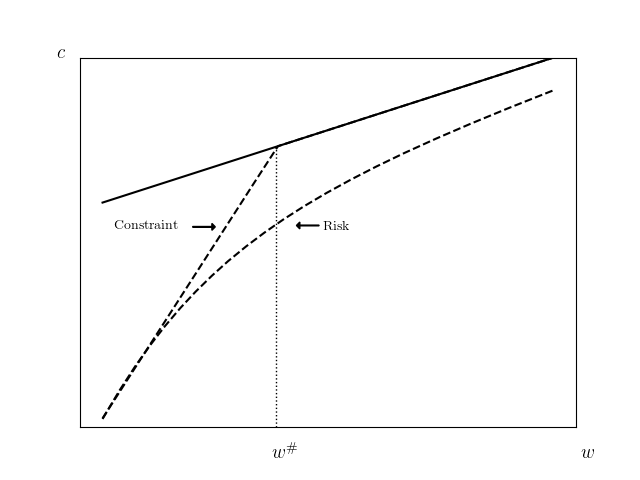
\includegraphics[width=.95\textwidth]{\FigDir/CounterclockwiseConcavifications}}
	\caption{Examples of Counterclockwise Concavifications}
	{\footnotesize \begin{singlespace} {\emph{Notes:} The solid line shows the linear consumption function in the case with no constraints and no risks. The two dashed line show the consumption function when we introduce a constraint and a risk, respectively. The introduction of a constraint is a counterclockwise concavification of the solid consumption function around $w^{\#}$, while the introduction of a risk is a counterclockwise concavification around $\infty$.}  \end{singlespace}}
	\label{fig:counterclockwise}
\end{figure}


\subsection{Consumption Concavity and Prudence}
The section above established all the tools necessary to show the relationship between consumption concavity and prudence. Our method in this section is to compare prudence in a \textit{baseline} case where the consumption function is $c(w)$ to prudence in a \textit{modified} situation in which the consumption function $\hat{c}(w)$ is a counterclockwise concavification of the baseline consumption function.

\begin{theorem}\label{thm:CCToPrud}  (Counterclockwise Concavification and Prudence). \\
	Consider an agent who has a utility function %of the HARA class \eqref{eq:HARA}
	with $u' > 0$, $u'' < 0$, $u''' \geq 0$, and non-increasing absolute prudence $-u'''/u''$. If $c(w)$ is concave and $\hat{c}(w)$ is a counterclockwise concavification of $c(w)$, then the value function associated with $\hat{c}(w)$ exhibits greater prudence than the value function associated with $c(w)$ for all $w$.
\end{theorem}
\noindent See Appendix \ref{app:CCToPrud} for the proof.
There are two channels through which a counterclockwise concavification heightens prudence. First, if the absolute prudence of the utility function is non-increasing, then the reduction in consumption and increase in MPC from the counterclockwise concavification make households more prudent. Second, the increase in consumption concavity from the counterclockwise concavification itself also heightens prudence. The channels operate separately, implying that a counterclockwise concavification heightens prudence \textit{even if absolute prudence is zero} as in the quadratic case.

Theorem \ref{thm:CCToPrud} only provides conditions for when the value function exhibits greater prudence, but not strictly greater prudence. In particular, the value function associated with $\hat{c}(w)$ will in some cases exhibit equal prudence for many values of $w$ and strictly greater prudence only for some values of $w$. In Corollary \ref{cor:ccandstrictprud}, we provide conditions for when the value function exhibits strictly greater prudence.

\begin{corollary} \label{cor:ccandstrictprud}(Counterclockwise Concavification and Strictly Greater Prudence).\\
	Consider an agent who has a utility function with $u' > 0$, $u'' < 0$, $u''' \geq 0$, and non-increasing absolute prudence $-u'''/u''$. If $c(w)$ is concave and $\hat{c}(w)$ is a counterclockwise concavification of $c(w)$, then the value function associated with $\hat{c}(w)$ exhibits strictly greater prudence than the value function associated with $c(w)$ at $w$ if the utility function satisfies $u''' > 0$ and $w < w^{\#}$ (the point of counterclockwise concavification) or the utility function is quadratic ($u''' = 0$) and $\frac{\hat{c}'(w)}{c'(w)}$ strictly declines at $w$.
\end{corollary}
\noindent See Appendix \ref{app:ccandstrictprud} for the proof. For prudent households ($u''' > 0$), the value function exhibits strictly greater prudence for all levels of wealth where the counterclockwise concavification affects consumption. This is a result of the fact that a reduction in consumption and higher marginal propensity to consume heighten prudence if the utility function has a positive third derivative and prudence is non-increasing. If the utility function instead is quadratic, the third derivative is zero and the absolute prudence of the utility function does not depend on the level of consumption or the marginal propensity to consume. In this case, the counterclockwise concavification only affects prudence at the kink points in the consumption function, i.e. where $\frac{\hat{c}'(w)}{c'(w)}$ strictly declines at $w$.


\section{Recursive Propagation of Consumption Concavity}\label{sec:Aggregation} 

  
In section \ref{sec:PrudAndCC}, we provide conditions for when consumption concavity heightens prudence by comparing value functions and consumption functions at a specific point in time. In this section, we provide conditions guaranteeing that if the consumption function is concave in period $t+1$, it will be concave in period $t$ and earlier, whatever the source of that concavity may be.

\begin{theorem}\label{thm:recursive}(Recursive Propagation of Consumption Concavity). \\
	Consider an agent with a HARA utility function satisfying $u' > 0$, $u'' < 0$, $u''' \geq 0$ and non-increasing absolute prudence $-u'''/u''$. Assume that no liquidity constraint applies at the end of period $t$ and that the agent faces income risk $y_{t+1} \in [\underline{y},\bar{y}]$. If $V_{t+1}(w_{t+1})$ exhibits property consumption concavity for all $w_{t+1} \in [Rs_t + \underline{y}, Rs_t + \bar{y}]$, then $V_t(w_t)$ exhibits property consumption concavity at the level of wealth $w_t$ such that optimal consumption yields $s_t = w_t - c_t(w_t)$.

	\medskip
	If also $V_{t+1}(w_{t+1})$ exhibits property strict consumption concavity for at least one $w_{t+1} \in [Rs_t + \underline{y}, Rs_t + \bar{y}]$, then $V_t(w_t)$ exhibits property strict consumption concavity at the level of wealth $w_t$ where optimal consumption yields $s_t = w_t - c_t(w_t)$.
\end{theorem}
See Appendix \ref{app:recursive} for the proof. Theorem \ref{thm:recursive} presents conditions to ensure that the consumption function is concave today if the consumption function is concave in the future. The basic insight is that as long as the future consumption function is concave for all realization of $y_{t+1}$, then it is also concave today. Additionally, if the
the future consumption function is strictly concave for at least one realization of ${y}_{t+1}$, then the consumption function is strictly concave also today. 


\section{Liquidity Constraints and Consumption Concavity}\label{sec:Precaution} 

We now move on to the sources of consumption concavity. In our setting, there are two sources of consumption concavity: risk and constraints. The properties of consumption under risk have already been derived in \citet{carroll&kimball:concavity}. We therefore restrict our attention to showing how liquidity constraints make the consumption function concave. Once the relationship between liquidity constraints and consumption concavity is established, we use the results on consumption concavity and prudence to show under which conditions liquidity constraints increase prudence.

\subsection{Notation}
Throughout this paper, we are working with a finite horizon household with an horizon going from $0$ to $T$. A liquidity constraint is a constraint on wealth that binds at a specific time $t \in (0, T]$. We first define an ordered set to keep track of the liquidity constraints.
\begin{defn} (The Set of Liquidity Constraints). \\
	We define $\mathcal{T}$ as an ordered set of dates at which a relevant constraint exists. We define $\mathcal{T}[1]$ as the last period in which a constraint exists, and $\mathcal{T}[2]$ is the date of the last period before $\mathcal{T}[1]$ in which a constraint exists, and so on.
\end{defn}
For any $t \in [0, T)$, we define $c_{t,n}$ as the optimal consumption function in period $t$ assuming that the first $n$ constraints in $\mathcal{T}$ have been imposed. For example, $c_{t,0}(w)$ is the consumption function in period $t$ when no constraint (aside from the intertemporal budget constraint) has been imposed, $c_{t,1}(w)$ is the consumption function in period $t$ after the chronologically last constraint has been imposed, and so on. We define $\Omega_{t,n}, V_{t,n}$, and other functions correspondingly.

To have a distinct terminology for the effects of current-period and future-period constraints, we will restrict the use of the term `binds' to the potential effects of a constraint in the period in which it applies (`the constraint binds if wealth is less than ...') and will use the term `impinges' to describe the effect of a future constraint on current consumption. We can now define the concept of a kink point.
\begin{defn}(Kink Point). \\
	We define a kink point, $\wAlt_{t,n}$ as the level of wealth at which constraint $n$ stops binding (impinging) on time $t$ consumption.
\end{defn}
A kink point corresponds to a transition from a level of wealth where a current constraint binds or a future constraint impinges, to a level of wealth where that constraint no longer binds or impinges.



\subsection{Perfect Foresight Consumption with Liquidity Constraint}\label{subsec:Piecewise}

We first consider an initial situation in which a consumer is solving a perfect foresight optimization problem with a finite horizon that begins in period $t$ and ends in period $T$. The consumer begins with wealth $w_{t}$ and earns constant income ${y}$ in each period. Wealth accumulates according to $w_{t+1} = Rs_{t}+{y}$. We are interested in how this consumer's behavior in period $t$ changes from an initial situation with $n\geq 0$ constraints to a situation in which $n+1$ liquidity constraints has been imposed.

\begin{theorem}\label{thm:pfclc}(Perfect Foresight Consumption with Liquidity Constraints). \\
	Consider an agent who has a utility function with $u'> 0 $ and $u'' < 0$, faces constant income ${y}$, and is `absolutely impatient' (by which we mean $\beta R < 1$). Assume that the agent faces a set $\mathcal{T}$ of $N$ relevant constraints. Then $c_{t,n+1}(w)$ is a counterclockwise concavification of $c_{t,n}(w)$ around $\wAlt_{t,n+1}$ for all $n \leq N-1$
\end{theorem}

See Appendix \ref{app:pfclc} for the proof. Theorem \ref{thm:pfclc} shows that when we have an ordered set of constraints, $\mathcal{T}$, the introduction of the next constraint in the set represents a counterclockwise concavification of the consumption function. Note that constraint $n+1$ is always at a date prior to the set of the $n$ first constraints. From the proof of Theorem \ref{thm:pfclc}, we also know the shape of the perfect foresight consumption function with liquidity constraints:

\begin{corollary}(Piecewise Linear Consumption Function). \\
	Consider an agent who has a utility function with $u'> 0$ and $u'' < 0$, faces constant income ${y}$, and is absolutely impatient. Assume that the agent faces a set $\mathcal{T}$ of $N$ relevant constraints. When $n \leq N$ constraints have been imposed, $c_{t,n}(w)$ is a piecewise linear increasing concave function with kink points at successively larger values of wealth at which future constraints stop impinging on current consumption.
\end{corollary}

Since the consumption function is piecewise linear, the new consumption function, $c_{t,n+1}(w)$ is not necessarily strictly more concave than $c_{t,n}(w)$ for all $w$. This is where the concept of counterclockwise concavification is useful. Even though $c_{t,n+1}(w)$ is not strictly more concave than $c_{t,n}(w)$ everywhere, it is a counterclockwise concavification and we apply Theorem \ref{thm:CCToPrud} to derive the consequences of imposing one more constraint on prudence.

\begin{theorem}\label{thm:lcip} (Liquidity Constraints Increase Prudence). \\
	Consider an agent in period $t$ who has a utility function with $u' > 0$, $u'' < 0$, $u''' \geq 0$ and non-increasing absolute prudence $-u'''/u''$, faces constant income ${y}$, and is impatient, $\beta R < 1$. Assume that the agent faces a set $\mathcal{T}$ of $N$ relevant constraints. When $n \leq N-1$ constraints have been imposed, the imposition of constraint $n+1$ strictly increases absolute prudence of the agent's value function if $u''' > 0$ and $w_t < \wAlt_{t,n+1}$ or if $u''' = 0$ and $\frac{c'_{t,n+1}}{c'_{t,n}}$ strictly declines at $w$.
\end{theorem}
\begin{proof}
	By Theorem \ref{thm:pfclc}, the imposition of constraint $n+1$ constitutes a counterclockwise concavification of $c_{t,n}(w)$. By Theorem \ref{thm:CCToPrud} and Corollary \ref{cor:ccandstrictprud}, such a concavification strictly increases absolute prudence of the value function for the cases in Corollary \ref{cor:ccandstrictprud}.
\end{proof}

Theorem \ref{thm:lcip} is the main result in the current section: the introduction of the next liquidity constraint increases absolute prudence of the value function. In the subsequent discussions, we consider cases where we relax the assumptions underlying Theorem \ref{thm:lcip}. We first consider the case where we add an extra constraint to the set of relevant constraints. Next, we consider the cases with time-varying deterministic income, general constraints, and no assumption on time discounting.






\subsection{Increasing the Number of Constraints}
\label{subsec:IncreaseNumConstr}

In the previous section, we analyzed a case where there was a preordained set
of constraints $\mathcal{T}$ which were applied sequentially.  We now examine how behavior will be modified if we add a new date to the set of dates at which the consumer is constrained.

Call the new set of dates $\hat{\mathcal{T}}$ with $N+1$ constraints (one more constraint than before), and call the consumption rules corresponding to the new set of dates
$\hat{c}_{t,1}$ through $\hat{c}_{t,N+1}$. Now call $m$ the
number of constraints in $\mathcal{T}$ at dates strictly
greater than $\hat{\tau}$.  Then note that that $\hat{c}_{\hat{\tau},m} =
c_{\hat{\tau},m}$, because at dates after the date at which the new constraint (number $m+1$) is
imposed, consumption is the same as in the absence of the new constraint.
Now recall that imposition of the constraint at $\hat{\tau}$ causes a counterclockwise concavification of the consumption function around a new kink point, $\wAlt_{\hat{\tau},m+1}$. That is, $\hat{c}_{\hat{\tau},m+1}$ is a counterclockwise concavification of $\hat{c}_{\hat{\tau},m} = c_{\hat{\tau},m}$.

The most interesting observation, however, is that behavior under constraints $\hat{\mathcal{T}}$ in periods strictly before $\hat{\tau}$ \textit{cannot} be described as a counterclockwise concavification of behavior under $\mathcal{T}$.  The reason is that the values of wealth at which the earlier constraints caused kink points in the consumption functions before period $\hat{\tau}$ will not generally correspond to kink points once the extra constraint has been added.

\hypertarget{CurrConstrHidesFutKink}{}

\begin{figure}[ht]
{\centering 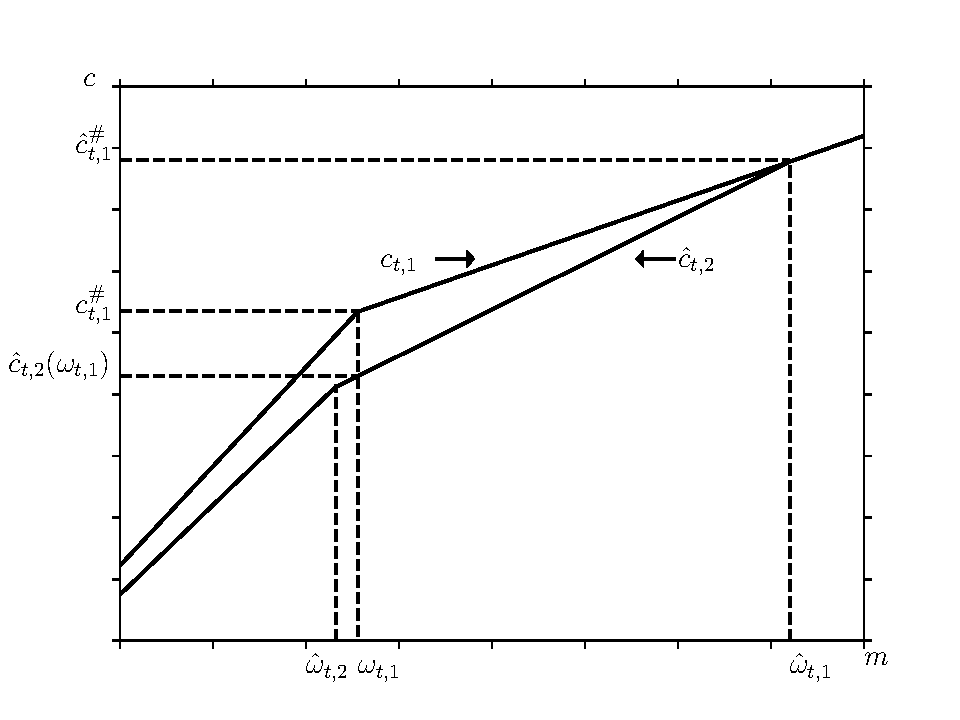
\includegraphics[width=.95\textwidth]{\FigDir/CurrConstrHidesFutKink}}
\caption{How a future constraint can `hide' a current kink}
\footnotesize {\emph{Notes:} $c_{t,1}$ is the original consumption function with one constraint that induces a kink point at $\omega_{t,1}$. $\hat{c}_{t,2}$ is the modified consumption function in where we have introduced one new constraint. The two constraints affect $\hat{c}_{t,2}$ through two kink points: $\hat{\omega}_{t,1}$ and $\hat{\omega}_{t,2}$. Since we introduced the new constraint at a later point in time than the current existing constraint, the future constraint affects the position of the kink induced by the current constraint and the modified consumption function $\hat{c}_{t,2}$ is not a counterclockwise concavification of ${c}_{t,1}$.}
\label{fig:LCtHidesLCtpn}
\end{figure}

We present an example in Figure~\ref{fig:LCtHidesLCtpn}. The original $\mathcal{T}$ contains only a single constraint, at the end of period $t+1$, inducing a kink point at $\wAlt_{t,1}$ in the consumption rule $c_{t,1}$. The expanded set of constraints, $\hat{\mathcal{T}}$, adds one constraint at period $t+2$. $\hat{\mathcal{T}}$ induces two kink points in the updated consumption rule $\hat{c}_{t,2}$, at $\hat{\wAlt}_{t,1}$ and $\hat{\wAlt}_{t,2}$.  It is true that imposition of the new constraint causes consumption to be lower than before at every level of wealth below $\hat{\wAlt}_{t,1}$.  However, this does not imply higher prudence of the value function at every $w <\hat{\wAlt}_{t,1}$.  In particular, note that the original consumption function is strictly concave at $w = \wAlt_{t,1}$, while the new consumption function is linear at $\wAlt_{t,1}$, so prudence can be greater before than after imposition of the new constraint at this particular level of wealth.

The intuition is simple: At levels of initial wealth below $\hat{\wAlt}_{t,1}$, the consumer had been planning to end period $t+2$ with negative wealth. With the new constraint, the old plan of ending up with negative wealth is no longer feasible and the consumer will save more for any given level of current wealth below $\hat{\wAlt}_{t,1}$, including $\wAlt_{t,1}$. But the reason $\wAlt_{t,1}$ was a kink point in the initial situation was that it was the level of wealth where consumption would have been equal to wealth in period $t+1$. Now, because of the extra savings induced by the constraint in $t+2$, the larger savings induced by wealth $\wAlt_{t,1}$ implies that the period $t+1$ constraint will no longer bind for a consumer who begins period $t$ with wealth $\wAlt_{t,1}$. In other words, at wealth $\wAlt_{t,1}$ the extra savings induced by the new constraint `hides' the original constraint and prevents it from being relevant any more at $\wAlt_{t,1}$.

Notice, however, that all constraints that existed in $\mathcal{T}$ will remain relevant at \textit{some} level of wealth under $\hat{\mathcal{T}}$ even after the new constraint is imposed - they just induce kink points at different levels of wealth than before, e.g. the first constraint causes a kink at $\hat{\wAlt}_{t,1}$ rather than at $\wAlt_{t,1}$.

\subsection{A More General Analysis}
\label{subsubsec:MoreGenConstr}

We now want to allow time variation in the level of income, ${y}_{t},$ and in the location of the liquidity constraint (e.g$.$ a constraint in period $t$ might require the consumer to end period $t$ with savings $s_{t}$ greater than $\sConst$ where $\sConst$ is a negative number).  We also drop the restriction that $\beta R < 1$, allowing the consumer to want to have consumption growth over time.

Under these more general circumstances, a constraint imposed in a given period can render constraints in either earlier or later periods irrelevant.  For example, consider a CRRA utility consumer with $\beta R=1$ who earns income of 1 in each period, but who is required to arrive at the end of period $T-2$ with savings of 5.  Then a constraint that requires savings to be greater than zero at the end of period $T-3$ will have no effect because the consumer is required by the constraint in period $T-2$ to end period $T-3$ with savings greater than 4. 

Formally, consider now imposing the first constraint, which applies in period $\tau < T$.  The simplest case, analyzed before, was a constraint that requires the minimum level of end-of-period wealth to be $s_{\tau} \geq 0$.  Here we generalize this to $s_{\tau} \geq \sConst_{\tau,2}$ where in principle we can allow borrowing by choosing $\sConst$ to be a negative number.  Now for constraint $2$ calculate the kink points for prior periods from
\begin{eqnarray}
  \label{eq:5}
  u'(c_{\tau,2}^{\#}) & = & R\beta u'(c_{\tau+1,1}(R\sConst_{\tau,1}+{y}_{t+1}))
\\ \wAlt_{\tau,2} & = & (V_{\tau,1}')^{-1}(u'(c_{\tau,2}^{\#})).
\end{eqnarray}
In addition, for constraint $2$ recursively calculate
\begin{eqnarray}
\underline{\sConst}_{\tau,2} & = & (\sConst_{\tau+1,2}-{y}_{\tau+1,2}+\underline{c})/R  \label{eq:cgt0}
\end{eqnarray}
where $\underline{c}$ is the lowest value of consumption permitted by the model (independent of constraints).\footnote{For example, CRRA utility is well defined only on the positive real numbers, so for a CRRA utility consumer $\underline{c}=0$.  In other cases, for example with exponential or quadratic cases, there is nothing to prevent consumption of $-\infty$, so for those models $\underline{c}=-\infty$, unless there is a desire to restrict the model to positive values of consumption, in which case the $c\geq 0$ constraint will be implemented through the use of \eqref{eq:cgt0}.}

Now assume that the first $n$ constraints in $\mathcal{T}$ have been imposed, and consider imposing constraint number $n+1$, which we assume applies in period $\tau$.  The first thing to check is whether constraint number $n+1$ is relevant given the already-imposed set of constraints.  This is simple: A constraint that requires $s_{\tau} \geq \sConst_{\tau,n+1}$ will be irrelevant if $\min_{i} [\underline{\sConst}_{\tau,i}] \leq \sConst_{\tau,n+1}$.  If the constraint is irrelevant then the analysis proceeds simply by dropping this constraint and renumbering the constraints in $\mathcal{T}$ so that the former constraint $n+2$ becomes constraint $n+1$, $n+3$ becomes $n+2$, and so on.

Now consider the other possible problem: That constraint number $n+1$ imposed in period $\tau$ will render irrelevant some of the constraints that have already been imposed.  This too is simple to check: It will be true if the proposed $\sConst_{\tau,n+1} \geq \sConst_{\tau,i}$ for any $i \leq n$.  The fix is again simple: Counting down from $i=n$, find the smallest value of $i$ for which $\sConst_{\tau,n+1} \geq \sConst_{\tau,i}$.  Then we know that constraint $n+1$ has rendered constraints $i$ through $n$ irrelevant. The solution is to drop these constraints from $\mathcal{T}$ and start the analysis over again with the modified $\mathcal{T}$. 

If this set of procedures is followed until the chronologically earliest relevant constraint has been imposed, the result will be a $\mathcal{T}$ that contains a set of constraints that can be analyzed as in the simpler case.  In particular, proceeding from the final $\mathcal{T}[1]$ through $\mathcal{T}[N]$, the imposition of each successive constraint in $\mathcal{T}$ now causes a counterclockwise concavification of the consumption function around successively lower values of wealth as progressively earlier constraints are applied and the result is again a piecewise linear and strictly concave consumption function with the number of kink points equal to the number of constraints that are relevant at any feasible level of wealth in period $t$.

The preceding discussion thus establishes the following result:
\begin{theorem}\label{thm:lcip2} (Liquidity Constraints Increase Prudence). \\
	Consider an agent in period $t$ who has a utility function with $u' > 0$, $u'' < 0$, $u''' \geq 0$, and non-increasing absolute prudence $-u'''/u''$. Assume that the agent faces a set $\mathcal{T}$ of $N$ relevant constraints. When $n \leq N-1$ constraints have been imposed, the imposition of constraint $n+1$ strictly increases absolute prudence of the agent's value function if the utility function satisfies $u''' > 0$ and $w_t < \wAlt_{t,n+1}$ or if $u''' = 0$ and $\frac{c'_{t,n+1}}{c'_{t,n}}$ strictly declines at $w$.
\end{theorem}

Theorem \ref{thm:lcip2} is a generalization of Theorem \ref{thm:lcip}. Even if we relax the assumptions that income is constant and the agent is impatient, the imposition of an extra constraint increases absolute prudence of the value function as long as we are careful when we select the set $\mathcal{T}$ of relevant constraints.

Finally, consider adding a new constraint to the problem and call the new set of constraints $\hat{\mathcal{T}}$.  Suppose the new constraint applies in period $\hat{\tau}$.  Then the analysis of the new situation will be like the analysis of an added constraint in the simpler case in section \ref{subsec:IncreaseNumConstr} if the new constraint is relevant given the constraints that apply after period $\hat{\tau}$ and the new constraint does not render any of those later constraints irrelevant. If the new constraint fails either of these tests, the analysis of $\hat{\mathcal{T}}$ can proceed from the ground up as described above.


\section{Liquidity Constraints and Precautionary Saving}
\label{sec:ConstrRisksCPPandPS}

In the three previous sections, we have derived the relationships between liquidity constraints, consumption concavity, and prudence. It is now time to be explicit about the last step: the relationship between liquidity constraints and precautionary saving. We first explain the relationship between the precautionary premium and absolute prudence. In the next subsection, we use this result to show how the introduction of an additional constraint induces households to increase precautionary saving when they face a current risk. Next, we explain why the result cannot be generalized to the cases with risks in different time periods or earlier constraints. We end this section by showing our most general result on liquidity constraints and precautionary saving: The introduction of a risk has a greater precautionary effect on consumption in the presence of all future risks and constraints than in the absence of any future risks or constraints.

\subsection{Notation}\label{subsec:PrudAndCPP}

We begin by defining two marginal value functions $V'(w)$ and $\hat{V}'(w)$ which are convex, downward sloping, and continuous in wealth, $w$. We consider a risk $\zeta$ with support $[\underline{\zeta},\bar{\zeta}]$, and follow \citet{kimball:smallandlarge} by defining the Compensating Precautionary Premia (CPP) as the values $\kappa$ and $\hat{\kappa}$ such that
\begin{eqnarray}
V'(0) & = & \Ex[V'(\zeta + \kappa)] \label{eq:mudef}
\\ \hat{V}'(0) & = & \Ex[\hat{V}'(\zeta + \hat{\kappa})] \label{eq:checkmudef}.
\end{eqnarray}
The CPP can be interpreted as the additional resources an agent requires to be indifferent between accepting the risk and not accepting the risk. The relevant part of \citet{pratt:smallandlarge}'s Theorem 1 as reinterpreted using \citet{kimball:smallandlarge}'s Lemma (p. 57) can be restated as
\begin{lemma}\label{lemma:kimpratt}
	Let $A(w)$ and $\hat{A}(w)$ be absolute prudence of the value functions $V$ and $\hat{V}$ respectively at $w$,\footnote{A small technicality: Absolute prudence of value functions is infinite at kink points in the consumption function, so if both $c(w)$ and $\hat{c}(w)$ had a 		kink point at exactly the same $w$ but the amount by which the slope declined were different, the comparison of prudence would not yield a well-defined answer.  Under these circumstances we will say that $\hat{A}(w) > A(w)$ if the decline in the MPC is greater for $\hat{c}$ at $w$ than for $w$. } and let $\kappa$ and $\hat{\kappa}$ be the respective compensating precautionary premia associated with imposition of a given risk $\zeta$ as per \eqref{eq:mudef} and \eqref{eq:checkmudef}. Then the following conditions are equivalent:
	\begin{enumerate}
		\item $\hat{A}(\zeta+\kappa) \geq A(\zeta+\kappa)$ for all $\zeta \in [\underline{\zeta},\bar{\zeta}]$ and $\hat{A}(\zeta+\kappa) > A(\zeta+\kappa)$ for at least one [no] point $\zeta \in [\underline{\zeta},\bar{\zeta}]$.
		\item $\hat{\kappa} > [=] \kappa$ with repect to the same risk $\zeta \in [\underline{\zeta},\bar{\zeta}]$.
	\end{enumerate}
\end{lemma}

Note finally that precautionary premia are not equivalent to precautionary saving effects because precautionary premia apply at a given level of consumption, while precautionary saving applies at a given level of wealth.

We now take up the question of how the introduction of a risk $\zeta_{t+1}$ that will be realized between period $t$ and $t+1$ affects consumption in period $t$ in the presence and in the absence of a subsequent constraint.  To simplify the discussion, consider a consumer for whom $\beta=R=1$, with mean income ${y}$ in $t+1$.

Assume that the realization of the risk $\zeta_{t+1}$ will be some value $\zeta$ with support [$\underline{\zeta}$,$\bar{\zeta}$], and signify a decision rule that takes account of the presence of the immediate risk by a $\sim$.  Thus, the perfect foresight unconstrained consumption function is $c_{t,0}(w)$, the perfect foresight consumption function in the presence of the future constraint is $c_{t,1}(w)$, the consumption function with no constraints but with the risk is $\tilde{c}_{t,0}(w)$ and the consumption function with both risk and constraint is $\tilde{c}_{t,1}(w),$ and similarly for the other functions. We now define two wealth levels that describe the subsets where constraint $n+1$ affects households at time $t$. The wealth limits corresponds to the levels of wealth where liquidity constraint $n+1$ never binds (1) and always binds (2) for a consumer facing income risk.

\begin{defn}(Wealth Limits).
	\begin{enumerate}
		\item ${\underline{\wAlt}}_{t,n+1}$ is the level of wealth such that an agent who faces risk $\zeta_{t+1}$ and $n+1$ constraints save so little that constraint $n+1$ will always bind in period $t+1$, defined as
	\begin{eqnarray}
	{\underline{\wAlt}}_{t,n+1} & = & \left(\tilde{V}_{t,n+1}'\right)^{-1}(\tilde{\Omega}_{t,n+1}^{\prime}(\wAlt_{t+1,n+1}-({y}+\bar{\zeta}))).
	\end{eqnarray}

	How to read these limits: $\wAlt_{t+1,n+1}$ is the level of wealth at which constraint $n+1$ starts binding in period $t+1$. $\wAlt_{t+1,n+1} - ({y} + \bar{\zeta})$ is then the level of wealth that ensures that constraint $n+1$ binds in period $t+1$ even with the best possible draw, $\bar{\zeta}$.

	\item ${\bar{\wAlt}}_{t,n+1}$ is the level of wealth such that an agent who faces risk $\zeta_{t+1}$ and $n+1$ constraints save enough to guarantee that constraint $n+1$ will never bind in period $t+1$, defined as
	\begin{eqnarray}
	{\bar{\wAlt}}_{t,n+1} & = & \left(\tilde{V}_{t,n+1}'\right)^{-1}(\tilde{\Omega}_{t,n+1}^{\prime}(\wAlt_{t+1,n+1}-({y}+\underline{\zeta}))) \label{eq:tildeomegabar}
	\end{eqnarray}

	\end{enumerate}
      \end{defn}

We must be careful to check that $\wAlt_{t+1,n+1}-({y}+\underline{\zeta})$ is inside the realm of feasible values of $s_{t}$, in the sense of values that permit the consumer to guarantee that future levels of consumption will be within the permissible range (e.g. positive for consumers with CRRA utility). If this is not true for some level of wealth, then any constraint that binds at or below that level of wealth is irrelevant, because the restriction on wealth imposed by the risk is more stringent than the restriction imposed by the constraint.


\subsection{Precautionary Saving with Liquidity Constraints}

We are now in the position to analyze the relationship between precautionary saving and liquidity constraints. Our first result regards the effect of an additional constraint on the precautionary saving of a household facing risk between period $t$ and $t+1$.

\begin{theorem}\label{thm:riskandconstraints} (Precautionary Saving with Liquidity Constraints). \\
	Consider an agent who has a utility function with $u'> 0$, $u''< 0$, $u''' > 0$, and non-increasing absolute prudence $-u'''/u''$, and that faces the risk, $\zeta_{t+1}$. Assume that the agent faces a set $\mathcal{T}$ of N relevant constraints and $n \leq N-1$. Then
	\begin{equation}
	c_{t,n+1}(w) - \tilde{c}_{t,n+1}(w) \geq c_{t,n}(w)-\tilde{c}_{t,n}(w), \label{eq:ineq}
	\end{equation}
	and the inequality is strict if $w_t < \bar{\wAlt}_{t,n+1}$.
\end{theorem}

See Appendix \ref{app:riskandconstraints} for the proof. Theorem \ref{thm:riskandconstraints} shows that the introduction of the next constraint induces the agent to reduce consumption in response to an immediate risk. Theorem \ref{thm:riskandconstraints} can be generalized to period $s < t$ if there is no risk or constraint between period $s$ and $t$. We just have to define $\bar{\wAlt}_{s,n+1}$ as the wealth level at which the agent will arrive in the beginning of period $t$ with wealth $\bar{\wAlt}_{t,n+1}$.

To illustrate the result in Theorem \ref{thm:riskandconstraints}, Figure~\ref{fig:SolveConstrCompare4Cases} shows an example of optimal consumption rules in period $t$ under different combinations of an immediate risk (realized between $t$ and $t+1$) and a future constraint (applying between periods $t+1$ and $t+2$).
\hypertarget{ConsWithWithoutConstrAndRisk}{}
\begin{figure}[ht]
	{\centering
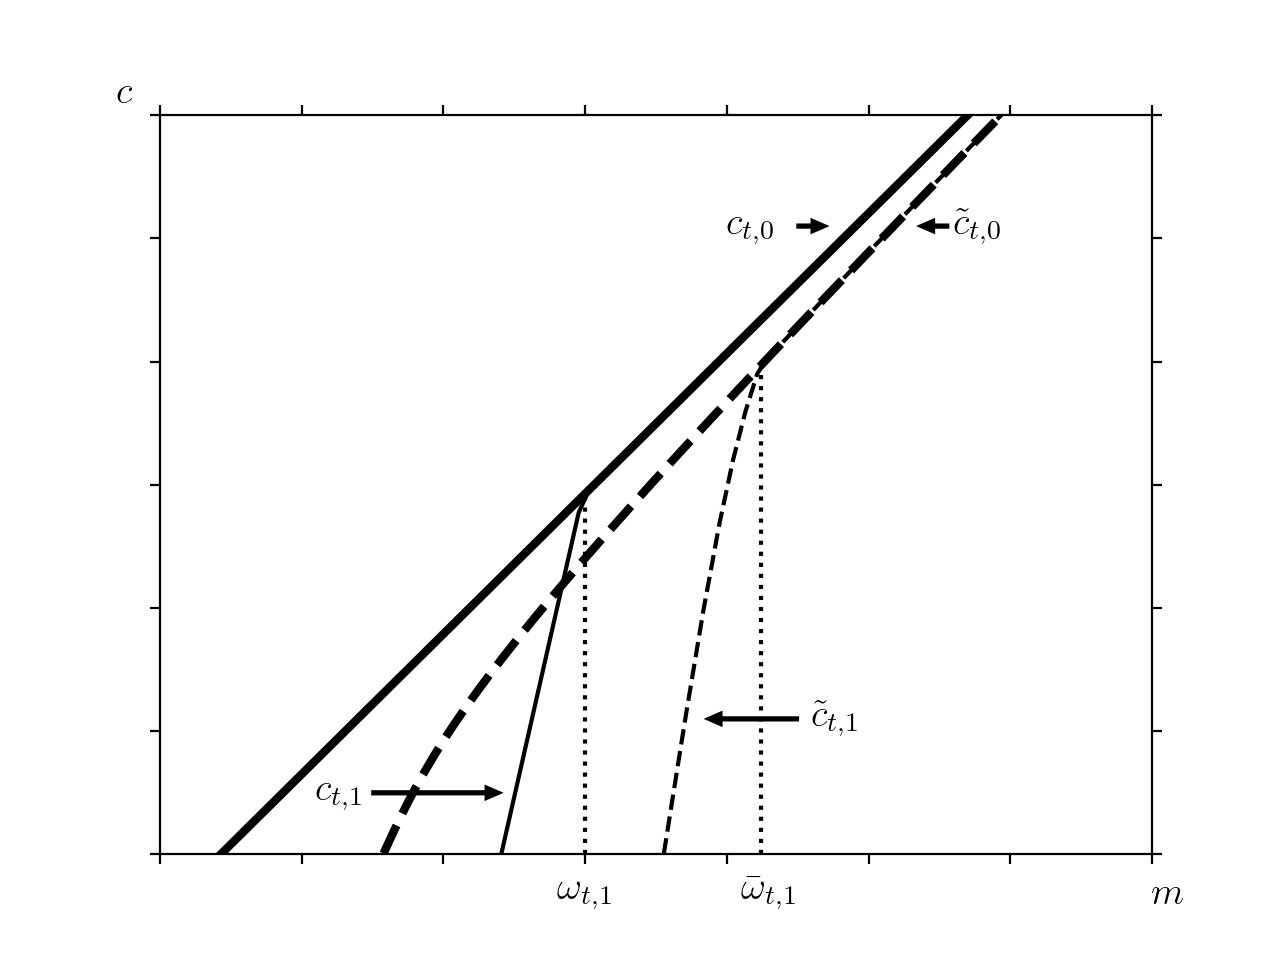
\includegraphics[width=.95\textwidth]{\FigDir/ConsWithWithoutConstrAndRisk}}

\caption{Consumption Functions with and without a Constraint and a Risk}
{\footnotesize \begin{singlespace} {\emph{Notes:} $c_{t,0}$ is the consumption function with no constraint and no risk, $\tilde{c}_{t,0}$ is the consumption function with no constraint and a risk that is realized between period $t$ and $t+1$, $c_{t,0}$ is the consumption function with one constraint in period $t+1$ and no risk, and $c_{t,0}$ is the consumption function with one constraint in period $t+1$ and a risk that is realized between period $t$ and $t+1$. The figure illustrates that the vertical distance between $c_{t,1}$ and $\tilde{c}_{t,1}$ is always greater than the vertical distance between $c_{t,0}$ and $\tilde{c}_{t,0}$ for $w < \bar{\omega}_{t,1}$. }  \end{singlespace}}
\label{fig:SolveConstrCompare4Cases}
\end{figure}
The darker loci reflect behavior of consumers who do not face the future constraint, and the dashed loci reflect behavior of consumers who \textit{do} face the immediate risk.  As expected, for levels of wealth above $\wAlt_{t,1}$ where the future constraint stops impinging on current behavior for perfect foresight consumers, behavior of the constrained and unconstrained perfect foresight consumers is the same. Similarly, $\tilde{c}_{t,1}(w_{t}) = \tilde{c}_{t,0}(w_{t})$ for levels of wealth above ${\bar{\wAlt}}_{t,1}$ beyond which the probability of the future constraint binding is zero. And for both constrained and unconstrained consumers, the introduction of the risk reduces the level of consumption (the dashed loci are below their solid counterparts). The importance of Theorem \ref{thm:riskandconstraints} in this context is that for levels of wealth below ${\bar{\wAlt}}_{t,1}$, the vertical distance between the solid and the dashed loci is greater for the constrained (thin line) than for the unconstrained (thick line) consumers, because of the interaction between the liquidity constraint and the precautionary motive.


\subsection{A More General Result?}
The results in Theorem \ref{thm:riskandconstraints} is limited to the effects of an additional constraint when a household faces income risk that is realized between period $t$ and $t+1$. We could hope to find a more general result where precautionary saving increases if we for example impose an immediate constraint or an earlier risk, or generally multiple constraints or risks. However, it turns out that the answer is "not necessary" to all these possible scenarios. In this subsection, we argue for why we cannot derive more general results.


To examine these results, we need to develop a last bit of notation.  We define, $c_{t,n}^{m}$, as the consumption function in period $t$ assuming that the first $n$ constraints and the first $m$ risks have been imposed, counting risks, like constraints, backwards from period $T$.  Thus, relating our new notation to our previous usage, $c_{t,n}^{0}=c_{t,n}$ because 0 risks have been imposed. All other functions are defined correspondingly, e.g. $\Omega_{t,n}^{m}$ is the end-of-period-$t$ value function assuming the first $n$ constraints and $m$ risks have been imposed. We will continue to use the notation $\tilde{c}_{t,n}$ to designate the effects of imposition of a single immediate risk (realized between periods $t$ and $t+1$).

Suppose now there are $m$ future risks that will be realized between $t$ and $T$. One might hope to show that the precautionary effect of imposing all risks in the presence of all constraints would be greater than the effect of imposing all risks in the absence of any
constraints:
\begin{equation}
  c_{t,n}^{0}(w) - c_{t,n}^{m}(w) \geq c_{t,0}^{0}(w) - c_{t,0}^{m}(w).\label{eq:nottrue}
\end{equation}
Such a hope, however, would be in vain.  In fact, we will now show that even the considerably weaker condition, involving only the single risk $\zeta_{t+1}$ and all constraints, $c_{t,n}^{0}(w) - c_{t,n}^{1}(w) \geq c_{t,0}^{0}(w) - c_{t,0}^{1}(w),$ can fail to hold for some $w$.


\subsubsection{An Immediate Constraint}\label{subsubsec:ImmediateConstr}


Consider a situation in which $n$ constraints applies in between $t$ and $T$. Since $c_{t,n-1}$ designates the consumption rule that will be optimal prior to imposing the period-$t$ constraint, the consumption rule imposing all constraints will be
\begin{eqnarray}
c_{t,n}(w) & = & \min[c_{t,n-1}(w),w].
\end{eqnarray}
Now define the level of wealth below which the period $t$ constraint binds for a consumer not facing the risk as ${\wAlt}_{t,n}.$ For values of wealth $w \geq {\wAlt}_{t,n},$ analysis of the effects of the risk is identical to analysis in the previous subsection where the first $n-1$ constraints were imposed. For levels of wealth $w < {\wAlt}_{t,n}$, we have $c^{1}_{t,n}(w) = c_{t,n}(w)=w$ (for the simple $c \leq w$
constraint; a corresponding point applies to the more sophisticated form of constraint); that is, for consumers with wealth below ${\wAlt}_{t,n}$, the introduction of the risk in period $t+1$ has no effect on consumption in $t$, because for these levels of wealth the constraint at the end of $t$ has the effect of `hiding' the
risk from view (they were constrained before the risk was imposed and remain constrained afterwards). Thus for households for whom inequality \eqref{eq:ineq} in Theorem \ref{thm:riskandconstraints} holds strictly in the absence of the constraint at $t$, at levels of wealth below ${\wAlt}_{t,n}$, the precautionary effect of the risk is wiped out.

\subsubsection{An Earlier Risk}\label{subsubsec:AnEarlierRisk}

Consider now the question of how the addition of a risk $\zeta_{t}$ that will be realized between periods $t-1$ and $t$ affects the consumption function at the beginning of period $t-1$, in the absence of any constraint at the beginning of period $t$.

The question at hand is then whether we can say that
\begin{eqnarray}
  \label{eq:earlierrisk}
  c_{t-1,0}^{1}(w)-c_{t-1,0}^{2}(w) & \geq & c_{t-1,0}^0(w)-c^{1}_{t-1,0}(w);
\end{eqnarray}
that is, does the introduction of the risk $\zeta_{t}$ have a greater precautionary effect on consumption in the presence of the subsequent risk $\zeta_{t+1}$ than in its absence?

The answer again is ``not necessarily.''  To see why, we present an example in Appendix \ref{app:similar} of a CRRA utility problem in which in a certain limit the introduction of a risk produced an effect on the consumption function that is indistinguishable from the effect of a liquidity constraint.  If the risk $\zeta_{t}$ is of this liquidity-constraint-indistinguishable form, then the logic of the previous subsection clearly applies: For some levels of wealth, the introduction of the risk at $t$ can `hide' the precautionary effect of any risks at $t+1$ or later.

\subsection{What Can Be Said?}\label{subsubsec:WhatCanBeSaid}



It might seem that the previous subsection implies that little useful can be said about the precautionary effects of introducing a new risk in the presence of preexisting constraints and risks. It turns out, however, that there is at least one useful result.

\begin{theorem}\label{thm:CCandPS}
	Consider an agent who has a utility function with $u'> 0$, $u''< 0$, $u''' > 0$, and non-increasing absolute prudence $-u'''/u''$. Then the introduction of a risk $\zeta_{t+1}$ has a greater precautionary effect on level $t$ consumption in the presence of all future risks and constraints than in the absence of any future risks and constraints, i.e.
	\begin{eqnarray}
	c_{t,n}^{m-1}(w) - c_{t,n}^{m}(w) & > & c_{t,0}^0(w)-c^{1}_{t,0}(w) \label{eq:whatcanbesaid}
	\end{eqnarray}
    at levels of period-$t$ wealth $w$ such that in the absence of the new risk the consumer is not constrained in the current period $(c_{t,n}^{m-1}(w) > w)$ and in the presence of the risk there is a positive probability that some future constraint will bind.
\end{theorem}

Appendix \ref{app:CCandPS} presents the proof. It seems to us that a fair summary of this theorem is that in most circumstances the presence of future constraints and risks does increase the amount of precautionary saving induced by the introduction of a given new risk.  The primary circumstance under which this should not be expected is for levels of wealth at which the consumer was constrained even in the absence of the new risk. There is no guarantee that the new risk will produce a sufficiently intense precautionary saving motive to move the initially-constrained consumer off his constraint.  If it does, the effect will be precautionary, but it is possible that no effect will occur.


\section{Conclusion}

The central message of this paper is that the effects of precautionary saving and of liquidity constraints are very similar to each other, because the introduction of either a liquidity constraints or of a risk induce counterclockwise concavifications of the consumption function. This increase in concavity increases prudence and induces households to save more for precautionary reasons. 

In addition, we provide an explanation of the apparently contradictory results that have emerged from simulation studies, which have sometimes seemed to indicate that constraints intensify precautionary saving motives, and sometimes have found constraints and precautionary behavior to be substitutes. The insight here is that the outcome depends on whether the introduction of a constraint or risk hides any previous constraints or risks. If the new constraint or risks does not hide existing constraints or risks, it intensifies the precautionary saving motive. If it hides any existing constraints or risks, it might weaken the precautionary saving motive.  

\bibliography{LiqConstr,LiqConstr-add,economics}

\vfill\eject
\appendix

  
\section{Proof of Lemma \ref{lem:counterclockwise}} \label{app:counterclockwise}
\begin{proof} First, condition 2 and 4 in Definition \ref{defn:cconcavification} implies that $\hat{c}'(w) > c'(w)$ for $w = w^{\#} - \epsilon$ for a small $\epsilon > 0$. Condition 3 then ensures that $\lim_{\upsilon \uparrow w} \hat{c}'(\upsilon) > \lim_{\upsilon \uparrow w} c'(\upsilon)$ holds for all $w \leq w^{\#}-\epsilon$ (equivalently $w < w^{\#}$). Second, condition 1 and the fact that $\lim_{\upsilon \uparrow w} \hat{c}'(\upsilon) > \lim_{\upsilon \uparrow w} c'(\upsilon)$ for $w < w^{\#}$ implies that $\lim_{\upsilon \uparrow w} \hat{c}(\upsilon) < \lim_{\upsilon \uparrow w}c(\upsilon)$ for $w < w^{\#}$. Third, condition 2 in Definition \ref{defn:cconcavification} implies that $$\lim_{\upsilon \uparrow w}\hat{c}''(\upsilon) \leq \lim_{\upsilon \uparrow w} c''(\upsilon)\frac{\hat{c}'(\upsilon)}{c'(\upsilon)}$$ for $w < w^{\#}$. Then $$\lim_{\upsilon \uparrow w} \hat{c}''(\upsilon) \leq \lim_{\upsilon \uparrow w} c''(\upsilon)$$ since $\lim_{\upsilon \uparrow w}\hat{c}'(\upsilon) > \lim_{\upsilon \uparrow w} c'(\upsilon)$ for $w < w^{\#}$. Note that the inequality is not strict since $c''(\upsilon)$ could be 0.  
\end{proof}



\section{Proof of Theorem \ref{thm:CCToPrud}} \label{app:CCToPrud}
\begin{proof}
	By the envelope theorem, we know that 
	\[ V'(w) = u'(c(w))\]
	Differentiating with respect to $w$ yields\footnote{Since $c(w)$ is concave, it has left-hand and right-hand derivatives at every point, though the left-hand and right-hand derivatives may not be equal. Equation \eqref{eq:diff2} should be interpreted as applying the left-hand and right-hand derivatives separately. (Reading \eqref{eq:diff2} in this way implies that $c'(w^-) \geq c'(w^+)$; therefore $V''(w^-) \leq V''(w^+)$).}
	\begin{equation}\label{eq:diff2}
	V''(w) = u''(c(w))c'(w)
	\end{equation}
	Taking another derivative can run afoul of the possible discontinuity in $c'(w)$ that we will show below can arise from liquidity constraints. We therefore consider two cases: (i) $c''(w)$ exists and (ii) $c''(w)$ does not exist. 
	
	\bigskip
	\noindent \textbf{\textit{Case I:}} ($c''(w)$ exists).\\
	In the case where $c''(w)$ exists, we can take another derivative
	\[V'''(w) = u'''(c(w))[c'(w)]^2 + u''(c(w))c''(w)\]
	Absolute prudence of the value function is thus defined as
	\begin{align}-\frac{V'''(w)}{V''(w)} &= -\frac{u'''(c(w))[c'(w)]^2 + u''(c(w))c''(w)}{u''(c(w))c'(w)} \nonumber \\
	-\frac{V'''(w)}{V''(w)} &= -\frac{u'''(c(w))}{u''(c(w))}c'(w) - \frac{c''(w)}{c'(w)}\label{eq:absprudence}\end{align}
	From the assumption that $\hat{c}(w)$ is a counterclockwise concavification of $c(w)$, we know from Lemma \ref{lem:counterclockwise} that  $\hat{c}(w) \leq c(w)$ and $\hat{c}'(w) \geq c'(w)$. Furthermore, since $-\frac{u'''(c(w))}{u''(c(w))}$ is non-increasing, we know that $-\frac{u'''(\hat{c}(w))}{u''(\hat{c}(w))} \geq -\frac{u'''(c(w))}{u''(c(w))}$. As a result, $-\frac{u'''(\hat{c}(w))}{u''(\hat{c}(w))}\hat{c}'(w) \geq -\frac{u'''(c(w))}{u''(c(w))}c'(w)$. 
	
	The second part of the absolute prudence expression, $-\frac{c''(w)}{c'(w)}$, is a measure of the curvature of the consumption function. Since the consumption function is concave, it is then a measure of the degree of concavity. Formally, if we have two functions, $f(x)$ and $g(x)$, that both are increasing and concave functions, then the concave transformation $g(f(x))$ always has more curvature.\footnote{To see this, calculate \[-\frac{\frac{d^2}{dx^2} g(f(x))}{\frac{d}{dx}g(f(x))} = - \frac{g''f'}{g'} - \frac{f''}{f'} \geq - \frac{f''}{f'}\] where the inequality holds since $g' \geq 0$ and $g'' \leq 0$.} A counterclockwise concavification is an example of such a $g$. Hence, $-\frac{\hat{c}''(w)}{\hat{c}'(w)} \geq -\frac{c''(w)}{c'(w)}$. Then
	\begin{align*}
	-\frac{\hat{V}'''(w)}{\hat{V}''(w)} &= -\frac{u'''(\hat{c}(w))}{u''(\hat{c}(w))}\hat{c}'(w) - \frac{\hat{c}''(w)}{\hat{c}'(w)} \\ 
	&\geq -\frac{u'''(c(w))}{u''(c(w))}c'(w) - \frac{c''(w)}{c'(w)} = -\frac{V'''(w)}{V''(w)}
	\end{align*}
	
	\bigskip
	\noindent \textbf{\textit{Case II:}} ($c''(w)$ does not exist).\\
	Informally, if nonexistence is caused by a constraint binding at $w$, the effect will be a discrete decline in the marginal propensity to consume at $w$, which can be thought of as $c''(w) = -\infty$, implying positive infinite prudence at that point (see \eqref{eq:absprudence}). Formally, if $c''(w)$ does not exist, greater prudence of $\hat{V}$ than $V$ is defined as $\frac{\hat{V}''(w)}{V''(w)}$ being a decreasing function of $w$. This is defined as
	\[\frac{\hat{V}''(w)}{V''(w)} \equiv 
	\left(\frac{u''(\hat c(w))}{u''(c(w))} \right)
	\left(\frac{\hat{c}'(w)}{c'(w)}\right)\]
	The second factor, $\frac{\hat{c}'(w)}{c'(w)}$, is weakly decreasing in $w$ by the assumption of counterclockwise concavity. At any specific value of $w$ where
	$\hat{c}''(w)$ does not exist because the left and right hand
	values of $\hat{c}'$ are different, we say that $\hat{c}'$
	is decreasing if
	\begin{eqnarray}
	\lim_{w^{-} \rightarrow w} \hat{c}'(w) & > & \lim_{w^{+} \rightarrow w} \hat{c}'(w).
	\end{eqnarray}
	
	As for the first factor, note that nonexistence of 	$\hat{V}'''(w)$ and/or $\hat{c}''(w)$ do not spring from nonexistence of either $u'''(c)$ or $\lim_{w \uparrow w} \hat{c}'(w)$ (for our purposes, when the left and right derivatives of $\hat{c}(w)$ differ at a point, the 	relevant derivative is the one coming from the left; rather than carry around the cumbersome limit notation, read the following derivation as
	applying to the left derivative).  To discover whether $\frac{\hat {V}''(w)}{V''(w)}$ is decreasing we can simply differentiate:
	\begin{align*}
	\frac{d}{d w}\left( \frac{u''(\hat{c}(w))}{ u''(c(w))}\right) &=& \frac{u'''(\hat{c}(w))\hat{c}'(w)u''(c(w))-u''(\hat{c}(w))u'''(c(w))c'(w)}{[u''(c(w))]^{2}}. \qquad \qquad
	\end{align*}
	
	Since the denominator is always positive, this will be negative if the numerator is negative, i.e.  if
	\begin{align}
	u'''(\hat{c}(w))u''(c(w))\hat{c}'(w) & \leq  u''(\hat{c}(w))u'''(c(w))c'(w) \nonumber
	\\  \frac{u'''(\hat{c}(w))}{u''(\hat{c}(w))}\hat{c}'(w) & \leq  \frac{u'''(c(w))}{u''(c(w))}c'(w) \nonumber
	\\  -\frac{u'''(\hat{c}(w))}{u''(\hat{c}(w))}\hat{c}'(w) & \geq  -\frac{u'''(c(w))}{u''(c(w))} c'(w) \label{eq:prudcond} .
	\end{align}
	
	Recall from Lemma \ref{lem:counterclockwise} that $\hat{c}'(w) \geq c'(w)$ and $\hat{c}(w) \leq c(w)$ so non-increasing absolute prudence of the utility function ensures that $-\frac{u'''(\hat{c}(w))}{u''(\hat{c}(w))} \geq  -\frac{u'''(c(w))}{u''(c(w))}$. Hence both terms on the LHS are greater than or equal to the corresponding terms on the RHS of equation \eqref{eq:prudcond}. 
	
\end{proof}



\section{Proof of Corollary \ref{cor:ccandstrictprud}} \label{app:ccandstrictprud}
\begin{proof}
	We prove each statement in Corollary \ref{cor:ccandstrictprud} separately. 
	
	\bigskip
	\noindent \textbf{\textit{Case I:}} ($ u ''' > 0$). \\
	If $u''' > 0$, a counterclockwise concavification around $w^{\#}$ implies that $\hat{c}(w) < c(w)$ and $\hat{c}'(w) > c'(w)$ for all $w < w^{\#}$. Then \[-\frac{u'''(\hat{c}(w))}{u''(\hat{c}(w)}\hat{c}'(w) > -\frac{u'''({c}(w))}{u''({c}(w))}{c}'(w) \text{ for } w < w^{\#} \]
	Since we know that \[-\frac{\hat{c}''(w)}{\hat{c}'(w)} \geq -\frac{{c}''(w)}{{c}'(w)} \text{ for } w < w^{\#}\]
	from the proof of Theorem \ref{thm:CCToPrud}, we know that
	\begin{align*}- \frac{\hat{V}'''(w)}{\hat{V}''(w)} &= -\frac{u'''(\hat{c}(w))}{u''(\hat{c}(w)}\hat{c}'(w) - \frac{\hat{c}''(w)}{\hat{c}'(w)}
	\\
	& > -\frac{u'''({c}(w))}{u''({c}(w))}{c}'(w) - \frac{{c}''(w)}{{c}'(w)} = - \frac{{V}'''(w)}{{V}''(w)} \text{ for } w < w^{\#}
	\end{align*}
	
	\bigskip
	\noindent \textbf{\textit{Case II:}} ($u''' = 0$). \\
	The quadratic case requires a different approach. Note first that the conditions in Corollary \ref{cor:ccandstrictprud} hold only below the bliss point for quadratic utility. In addition, since $u'''(\cdot) = 0$, strict inequality between the prudence of $\hat{V}$ and the prudence of $V$ hold only at those points where $\hat{c}(\cdot)$ is strictly concave. 
	
	Recall from the proof of Theorem \ref{thm:CCToPrud} that greater prudence of $\hat{V}(w)$ than $V(w)$ occurs if  $\frac{\hat{V}''(w)}{V''(w)}$ is decreasing in $w$. In the quadratic case
	\begin{equation}
	\frac{\hat{V}''(w)}{V''(w)} = \frac{u''(\hat{c}(w))}{u''(c(w))} \frac{\hat{c}'(w)}{c'(w)} = \frac{\hat{c}'(w)}{c'(w)}
	\end{equation}
	where the second equality follows since $u''(\cdot)$ is constant with quadratic utility. Thus, prudence is strictly greater in the modified case only if $ \frac{\hat{c}'(w)}{c'(w)}$ strictly declines in $w$.
\end{proof}

\section{Proof of Theorem \ref{thm:recursive}}\label{app:recursive}

\begin{proof}
	First, to facilitate readability of the proof, we assume that $R = \beta = 1$ with no loss of generality. Our goal is to prove that $V(w_t) \in CC$ if $V_{t+1}(s_t + {y}_{t+1}) \in CC$ for all realization of ${y}_{t+1}$. The proof proceeds in two steps. First, we show that property CC is preserved through the expectation operator (vertical aggregation),
	\[\Omega(s_t) = \Ex_t[V_{t+1}(s_t + {y}_{t+1})] \in CC,\]
	whenever $V_{t+1}(s_t + {y}_{t+1}) \in CC$ for all realization of ${y}_{t+1}$. Second, we show that property CC is preserved through the value function operator (horizontal aggregation),
	\[V(w_t) = \max_{s} u(c_t(w_t - s)) + \Omega(s) \in CC, \]
	whenever $\Omega(s) \in CC$. Throughout the proof, the first order condition holds with equality since no liquidity constraint applies at the end of period $t$. 
	
	\bigskip
	\noindent \textbf{Step 1: Vertical aggregation} \\ 
	\noindent We show that consumption concavity is preserved under vertical aggregation for three cases of the HARA utility function with $u''' \geq 0$ ($a \geq -1$) and non-increasing absolute prudence ($a \notin (-1,0)$). The three cases are
	\begin{equation}\label{eq:HARAmu}u'(c) = \begin{cases} \left(ac + b\right)^{-1/a} & a > 0 \text{ (CRRA)} \\
	e^{-c/b} & a = 0 \text{ (CARA)}\\
	ac + b & a = -1 \text{ (Quadratic)}\end{cases} \end{equation}
	
	\bigskip
	\noindent \textbf{Case I ($a > 0$, CRRA).} 	We will show that concavity is preserved under vertical aggregation for $c^{-1/a}$ to avoid clutter, but the results hold for all affine transformations, $ac + b$, with strictly positive $a$. Concavity of $c_{t+1}(s_t + \chi{y}_{t+1})$ implies that
	\begin{equation}c_{t+1}(s_t + {y}_{t+1}) \geq pc_{t+1}(s_1 + {y}_{t+1}) + (1-p) c_{t+1}(s_2 + {y}_{t+1}) \label{eq:vert_crra_conc}\end{equation}
	for all ${y}_{t+1} \in [\underline{y},\bar{y}]$ if $s_t = ps_1 + (1-p)s_2$ with $p \in [0,1]$. Since this holds for all ${y}_{t+1}$, we know that
	\[\left\{\Ex_t\left[c_{t+1}(s_t + \chi{y}_{t+1})^{-\frac{1}{a}}\right]\right\}^{-a} \geq \left\{\Ex_t\left[\left\{pc_{t+1}(s_1 + \chi{y}_{t+1}) + (1-p) c_{t+1}(s_2 + \chi{y}_{t+1})\right\}^{-\frac{1}{a}}\right]\right\}^{-a}\]
	
	By Minkowski's inequality, we know that for $a > 0$ $(a > -1, a \neq 0)$
	\[\left\{\Ex[(u + v)^{-\frac{1}{a}}]\right\}^{-a} \geq \left\{\Ex[u^{-\frac{1}{a}}]\right\}^{-a} + \left\{\Ex[v^{-\frac{1}{a}}]\right\}^{-a}\]
	if $u\geq 0$ and $v\geq 0$. Thus
	\begin{align*}
	&\left\{ \Ex_t \left[\left\{pc_{t+1}(s_1 + \chi{y}_{t+1}) + (1-p) c_{t+1}(s_2 + \chi{y}_{t+1})\right\}^{-\frac{1}{a}}\right]\right\}^{-a} \\ & \geq \left\{ \Ex_t \left[\left\{pc_{t+1}(s_1 + \chi{y}_{t+1})\right\}^{-\frac{1}{a}}\right]\right\}^{-a} + \left\{ \Ex_t \left[\left\{(1-p) c_{t+1}(s_2 + \chi{y}_{t+1})\right\}^{-\frac{1}{a}}\right]\right\}^{-a} \\
	& = p\left\{ \Ex_t \left[\left\{c_{t+1}(s_1 + \chi{y}_{t+1})\right\}^{-\frac{1}{a}}\right]\right\}^{-a} +(1-p) \left\{ \Ex_t \left[\left\{ c_{t+1}(s_2 + \chi{y}_{t+1})\right\}^{-\frac{1}{a}}\right]\right\}^{-a} \\ & = p(\Omega'(s_1))^{-a} + (1-p)(\Omega'(s_2))^{-a}
	\end{align*}
	which implies that 
	\[ (\Omega'(s_t))^{-a} \geq p(\Omega'(s_1))^{-a} + (1-p)(\Omega'(s_2))^{-a}\]
		
	Thus, defining
	$\chi_{t}(s_{t}) = \{\Omega_{t}^{'}(s_{t})\}^{-a}$, we get
	\begin{align*}
	\chi_{t}(s_{t}) \geq p \chi_{t}(s_{1}) + (1-p) \chi_{t}(s_{2})
	\end{align*}
	for all $s_{t}$, where the inequality is strict if $c_{t+1}$ is strictly concave for at least one realization of ${y}_{t+1}$.
	
	\bigskip
	\noindent \textbf{Case II ($a = 0$, CARA)}. For the exponential case, property CC holds at $s_{t}$ if 
	\begin{eqnarray*}
	\exp(-\chi_{t}(s_{t})/b) & = & \Ex_{t}[ \exp(-c_{t+1}(s_{t}+{y}_{t+1})/b)]
	\end{eqnarray*}
	for some $\chi_{t}(s_{t})$ which is strictly concave at $s_{t}$. We set $b = 1$ to reduce clutter, but results hold for $b \neq 1$. Consider first a case where $c_{t+1}$ is linear over the range of possible values of $s_{t}+{y}_{t+1}$, then 
	\begin{eqnarray}
	\chi_{t}(s_{t}) & = & -\log \Ex_{t}[e^{-c_{t+1}(s_{t}+{y}_{t+1})}] \nonumber 
	\\& = & -\log \Ex_{t}[e^{-(c_{t+1}(s_{t}+\bar{y})+({y}_{t+1}-\bar{y})c_{t+1}^{'})}] \nonumber
	\\ & = & c_{t+1}(s_{t}+\bar{y}) - \log \Ex_{t}[e^{-({y}_{t+1}-\bar{y}) c_{t+1}^{'}}] \label{eq:expcdrops}
	\end{eqnarray}
	which is linear in $s_{t}$ since the second term is a constant.  
	
	Now consider a value of $s_{t}$ for which $c_{t+1}(s_{t}+{y}_{t+1})$ is strictly concave for at least one realization of ${y}_{t+1}$. Global weak concavity of $c_{t+1}$ tells us that for every ${y}_{t+1}$
	\begin{eqnarray}
	-c_{t+1}(s_{t}+{y}_{t+1}) & \leq & -((1-p)c_{t+1}(s_1+{y}_{t+1})+pc_{t+1}(s_{2}+{y}_{t+1})) \nonumber
	\\ \Ex_{t}[e^{-c_{t+1}(s_{t}+{y}_{t+1})}] & \leq & \Ex_{t}[e^{-((1-p)c_{t+1}(s_1+{y}_{t+1})+pc_{t+1}(s_{2}+{y}_{t+1}))}]. \label{eq:expconc}
	\end{eqnarray}
	
	Meanwhile, the arithmetic-geometric mean inequality states that for positive $u$ and $v$, if $\bar u = \Ex_t [ u]$ and $\bar v = \Ex_t [ v]$, then
	\begin{equation*}
	\Ex_t\left[( u/\bar u)^p ( v/\bar v)^{1-p}\right] 
	\leq \Ex_t \left[p ( u/\bar u)+(1-p)( v/\bar v)\right] = 1, 
	\end{equation*}
	implying that 
	\begin{equation*}
	\Ex_t [ u^p  v^{1-p}] \leq \bar u^p \bar v^{1-p}, 
	\end{equation*}
	where the expression holds with equality only if $v$ is proportional to $u$.  Substituting in $u= e^{-c_{t+1}(s_1 + {y}_{t+1})}$ and $v = e^{-c_{t+1}(s_2 + {y}_{t+1})}$, this means that
	\begin{eqnarray*}
	\Ex_t [e^{-p c_{t+1}(s_1 + {y}_{t+1}) - (1-p)c_{t+1}(s_2 + {y}_{t+1})}] & \leq &
	\left\{ \Ex_t  [e^{- c_{t+1}(s_1 + {y}_{t+1})} ] \right\}^p \left\{ \Ex_t  [e^{- c_{t+1}(s_2 + {y}_{t+1})} ] \right\}^{1-p}
	\end{eqnarray*}
	and we can substitute for the LHS from \eqref{eq:expconc}, obtaining
	\begin{eqnarray}
	\Ex_{t}[e^{-c_{t+1}(s_{t}+{y}_{t+1})}] & \leq &
	\left\{ \Ex_t  [e^{- c_{t+1}(s_1 + {y}_{t+1})} ] \right\}^p 	\left\{ \Ex_t  [e^{- c_{t+1}(s_2 + {y}_{t+1})} ] \right\}^{1-p} \nonumber
	\\ 
	\log \Ex_{t}[e^{-c_{t+1}(s_{t}+{y}_{t+1})}] &\leq &
	p \log \Ex_t  [e^{-c_{t+1}(s_1 + {y}_{t+1})} ] 
	+ (1-p) \log \Ex_t  [e^{-c_{t+1}(s_2 + {y}_{t+1})} ]  \label{eq:expineq2} 
	\end{eqnarray}
	which holds with equality only when $e^{-c_{t+1}(s_{1}+{y}_{t+1})}/e^{-c_{t+1}(s_{2}+{y}_{t+1})}$ is a constant. This will only happen if 	$c_{t+1}(s_{1}+{y}_{t+1})-c_{t+1}(s_{2}+{y}_{t+1})$ is constant, which (given that the MPC is strictly positive everywhere) requires 	$c_{t+1}(s_{t}+{y}_{t+1})$ to be linear for ${y}_{t+1} \in (\underline{y},\bar{y})$. Hence, 
	\begin{eqnarray*}
	\chi_{t}(s_t) & \geq & p \chi_{t}(s_{1}) + (1-p) \chi_{t}(s_{2}).
	\end{eqnarray*}
	where the inequality is strict for an $s_{t}$ from which $c_{t+1}$ is strictly concave for some realization of ${y}_{t+1}$.
		
	\bigskip
	\noindent \textbf{Case III ($a = -1$, Quadratic)}.
	In the quadratic case, linearity of marginal utility implies that
	\begin{eqnarray*}
	u'(\chi_{t}(s_{t})) & = & \Ex_{t}[u'(c_{t+1}(s_{t}+{y}_{t+1}))]
	\\   \chi_{t}(s_{t}) & = & \Ex_{t}[c_{t+1}(s_{t}+{y}_{t+1})]
	\end{eqnarray*}
	so $\chi_{t}$ is simply the weighted sum of a set of
	concave functions where the weights correspond to the probabilities of the various possible outcomes for ${y}_{t+1}$. The sum of concave functions is itself concave. And if additionally the consumption function is strictly concave at any point, the weighted sum is also strictly concave.
	

	\bigskip
	\noindent \textbf{Step 2: Horizontal aggregation:} \\
	We now proceed with horizontal aggregation, namely how concavity is preserved through the value function operation. Assume that $\Omega_t(s_t) \in CC$ at point $s_t$, then the first order condition implies that
	\[\Omega_t'(s_t) = u'(\chi_t(s_t))\]
	for some monotonically increasing $\chi_t(s_t)$ that satisfies
	\begin{align}
	\chi_t(ps_1 + (1-p)s_2) \geq p\chi_t(s_1) + (1-p)\chi_t(s_2) \label{eq:hor_conc}
	\end{align}
	for any $0 < p < 1$, and $s_1 < s_t < s_2$. % ($|s_2 - s_1|< \delta$ for any $\delta > 0$). 
	
	In addition, we know that the first order condition holds with equality such that $\Omega_t'(s_t) = u'(c_t(w_t)) = u'(\chi_t(s_t))$ which implies that $s_t = \chi_t^{-1}(c_t)$. Using this equation, we get
	\begin{align*}
	\chi_t(ps_1 + (1-p)s_2) &\geq p\chi_t(s_1) + (1-p)\chi_t(s_2) \\
	ps_1 + (1-p)s_2 &\geq \chi_t^{-1}(p\chi_t(s_1) + (1-p)\chi_t(s_2)) \\
	p\chi_t^{-1}(c_1) + (1-p)\chi_t^{-1}(c_2) &\geq \chi_t^{-1}(pc_1 + (1-p)c_2)
	\end{align*}
	which implies that $\chi_t^{-1}$ is a convex function. 
	
	Use the budget constraint to define
	\begin{align*}
	w_t &= s_t + c_t \\ 
	\wAlt(c_t) & = \chi^{-1}(c_t) + c_t
	\end{align*} 
	Now, since $\chi_t^{-1}$ is a convex function, and $\wAlt(c_t)$ is the sum of a convex and a linear function, it is also a convex function satisfying
	\begin{align}
	p\wAlt(c_1) + (1-p)\wAlt(c_2) &\geq \wAlt(pc_1 + (1-p)c_2) \nonumber \\
	\wAlt^{-1}(p\wAlt(c_1) + (1-p)\wAlt(c_2)) &\geq pc_1 + (1-p)c_2 \nonumber \\
	c(pw_1 + (1-p)w_2) &\geq pc(w_1) + (1-p)c(w_2) \label{eq:hor_conc2}
	\end{align} 
	so $c$ is concave.
	
	\bigskip
	\noindent \textbf{Strict Consumption Concavity.}
	When $V_{t+1}(w_{t+1})$ exhibits property strict consumption concavity for at least one $w_{t+1} \in [Rs_t + \underline{y}, Rs_t + \bar{y}]$, we know that $\chi_t(s_t)$ also exhibit property strict consumption concavity from the proof of vertical aggregation. Subsequently, equation \eqref{eq:hor_conc} holds with strict inequality, and this strict inequality goes through the proof of horizontal aggregation, implying that equation \eqref{eq:hor_conc2} holds with strict inequality. Hence, $c_t(w_t)$ is strictly concave if $c_{t+1}(s_t + {y}_{t+1})$ is concave for all realizations of ${y}_{t+1}$ and strictly concave for at least one realization of ${y}_{t+1}$. 
\end{proof}


\section{Proof of Theorem \ref{thm:pfclc}}\label{app:pfclc}
	We prove Theorem \ref{thm:pfclc} by induction in two steps. First, we show that all results in Theorem \ref{thm:pfclc} hold when we add the first constraint. The second step is then to show that the results hold when we go from $n$ to $n+1$ constraints. 	
	
	\begin{lemma}\textit{$(c_{t}' < c_{t+1}')$} \\
		Consider an agent who has a utility function with $u' > 0$ and $u'' < 0$, faces constant income, is impatient $\beta R < 1$, and has a finite life. Then $c_{t}' < c_{t+1}'$.
	\end{lemma}
	
	\begin{proof}
	The marginal propensity to consume in period $t$ can be obtained from the MPC in period $t+1$ from the Euler equation
	\begin{eqnarray*}
		u'(c_{t}(w_{t})) & =  & \beta R u'(c_{t+1}(R(w_{t}-c_{t}(w_{t}))+{y})).
	\end{eqnarray*}
	Differentiating both sides with respect to $w_{t}$ and omitting arguments to reduce
	clutter we obtain
	\begin{eqnarray*}
		u^{\prime\prime}(c_{t})c_{t}^{\prime} & =  & \beta R u^{\prime\prime}(c_{t+1})c_{t+1}^{\prime}R(1-c_{t}^{\prime}) \nonumber
		\\ \nonumber (u^{\prime\prime}(c_{t}) + \beta R u^{\prime\prime}(c_{t+1})c_{t+1}^{\prime}R)c_{t}^{\prime} & = & \beta R u^{\prime\prime}(c_{t+1})Rc_{t+1}^{\prime}
		\\ \frac{c_{t+1}^{\prime}}{c_{t}^{\prime}}   & = & \frac{u^{\prime\prime}(c_{t}) + \beta R u^{\prime\prime}(c_{t+1})c_{t+1}^{\prime}R}{\beta R u^{\prime\prime}(c_{t+1})R} \label{eq:mpcPF} \\
		\frac{c_{t+1}^{\prime}}{c_{t}^{\prime}}   & = & \frac{u^{\prime\prime}(c_{t})}{\beta R u^{\prime\prime}(c_{t+1})R} + c_{t+1}^{\prime} %\\ \frac{c_{t+1}^{\prime}}{c_{t}^{\prime}} & > &  1 
	\end{eqnarray*}
	Since $\beta R < 1$ ensures that $c_{t} > c_{t+1}$, we know that
	\[\frac{u^{\prime\prime}(c_{t})}{\beta R u^{\prime\prime}(c_{t+1})R} \geq  \frac{u^{\prime\prime}(c_{t+1})}{\beta R u^{\prime\prime}(c_{t+1})R} = \frac{1}{\beta R R} > \frac{1}{R}\]
	Furthermore, we know that
	\[c_{t}^{\prime} \geq \frac{R-1}{R}\]
	since $\frac{R-1}{R}$ is the MPC for an infinitely-lived agent with $\beta R = 1$. Hence, 
	\[\frac{c_{t+1}^{\prime}}{c_{t}^{\prime}} = \left(\frac{u^{\prime\prime}(c_{t})}{\beta R u^{\prime\prime}(c_{t+1})R} + c_{t}^{\prime} \right) > \frac{1}{R} + \frac{R-1}{R} = 1\]
	and it follows that $c_{t}^{\prime} <  c_{t+1}^{\prime}$.
	\end{proof}
	
	\begin{lemma}\label{lem:pfclc}(Consumption with one Liquidity Constraint). \\
		Consider an agent who has a utility function with $u'> 0 $ and $u'' < 0$, faces constant income, ${y}$, and is impatient, $\beta R < 1$. Assume that the agent faces a set $\mathcal{T}$ of one relevant constraint. Then $c_{t,1}(w)$ is a counterclockwise concavification of $c_{t,0}(w)$ around $\wAlt_{t,1}$.
	\end{lemma}
	
	
	\begin{proof}
	Define $\tau = \mathcal{T}[1]$, the time period of the constraint. Note first that consumption is unaffected by the constraint for all periods after $\tau$, i.e. $c_{\tau+k,1}=c_{\tau+k,0}$ for any $k > 0$. For period $\tau$ 	we can calculate the level of consumption at which the constraint binds by realizing that a consumer for whom the constraint binds will save nothing, and that the maximum amount of consumption at which the constraint binds will satisfy the Euler equation (only points where the constraint is strictly binding violate the Euler equation; the point on the cusp does not). Thus, we define $c_{\tau,1}^{\#}$ as the level of consumption in period $\tau$ at which the constraint stops binding, we have
	\begin{eqnarray*}
		\label{eq:ctau1}
		u'(c_{\tau,1}^{\#})   & = & \beta R u'(c_{\tau+1,0}({y}))
		\\   c_{\tau,1}^{\#}       & = & (u')^{-1}\left(\beta R u'(c_{\tau+1,0}({y}))\right),
	\end{eqnarray*}
	and the level of wealth at which the constraint stops binding can be obtained from
	\begin{eqnarray}
	\label{eq:omegaFromc}
	\wAlt_{\tau,1} & = & \left(V'_{\tau,1}\right)^{-1}(u'(c_{\tau,1}^{\#}))  .
	\end{eqnarray}
	
	Below this level of wealth, we have $c_{\tau,1}(w) = w$ so the MPC is one, while above it we have $c_{\tau,1}(w) = c_{\tau,0}(w)$ where the MPC equals the constant MPC for an unconstrained perfect foresight optimization problem with a horizon of $T-\tau$. Thus, $c_{\tau,1}$ satisfies our definition of a counterclockwise concavification of $c_{\tau,0}$ around $\wAlt_{\tau,1}$.  
	
	Further, we can obtain the value of period $\tau-1$ consumption at which the period $\tau$ constraint stops impinging on period $\tau-1$ behavior from
	\begin{eqnarray*}
		u'(c_{\tau-1,1}^{\#})   & = & \beta R u'(c_{\tau,1}^{\#}) \label{eq:ctaum1}
	\end{eqnarray*}
	and we can obtain $\wAlt_{\tau-1,1}$ via the analogue to \eqref{eq:omegaFromc}. Iteration generates the remaining $c_{.,1}^{\#}$ and $\wAlt_{.,1}$ values back to period $t$. 
	
Now consider the behavior of a consumer in period $\tau-1$ with a level of wealth $w<\wAlt_{\tau-1,1}$.  This consumer knows he will be constrained and will spend all of his resources next period, so at $w$ his behavior will be identical to the behavior of a consumer whose entire horizon ends at time $\tau$.  As shown in step I, the MPC always declines with horizon. The MPC for this consumer is therefore strictly greater than the MPC of the unconstrained consumer whose horizon ends at $T > \tau$.  Thus, in each period before $\tau+1$, the consumption function $c_{.,1}$ generated by imposition of the constraint constitutes a counterclockwise concavification of the unconstrained consumption function around the kink point $\wAlt_{.,1}$. 
	\end{proof}
	
	We have now shown the results in Theorem \ref{thm:pfclc} for $n = 0$. The last step is to show that they also hold for $n+1$ when it holds strictly for $n$. Consider imposing the $n+1$'th constraint and suppose for concreteness that it applies at the end of period $\tau$. It will stop binding at a level of consumption defined by
$$u'(c_{\tau,n+1}^{\#}) = \beta R u'(c_{\tau+1,n}({y})) = RBu'(y)$$ 
where the second equatility follows because a consumer with total resources $y$, constant income, and $\beta R < 1$ will be constrained. But note that by definition of $c^{\#}_{\tau,n}$, we obtain
	$$	u'(c_{\tau,n}^{\#})  =  (R \beta)^{\mathcal{T}[n]-\tau} u'({y})  <  R \beta u'({y}) = u'(c_{\tau,n+1}^{\#})$$
	where $\mathcal{T}[n]-\tau$ denotes the time remaining to the $n$'th constraint. Then, from the assumption of decreasing marginal utility, we know that
	\begin{eqnarray*}
		c_{\tau,n}^{\#} & \geq & c_{\tau,n+1}^{\#}.
	\end{eqnarray*}
	This means that the constraint is relevant: The pre-existing constraint $n$ does not force the consumer to do so much saving in period $\tau$ that the $n+1$'th constraint fails to bind.
	
	The prior-period levels of consumption and wealth at which constraint $n+1$ stops impinging on consumption can again be calculated recursively from
	\begin{eqnarray*}
		u'(c_{\tau,n+1}^{\#}) & = & R\beta u'(c_{\tau+1,n}({y}))
		\\  \wAlt_{\tau,n+1} & = & \left(V'_{\tau,n}\right)^{-1}(u'(c_{\tau,n+1}^{\#})).
	\end{eqnarray*}

	Furthermore, once again we can think of the constraint as terminating
	the horizon of a finite-horizon consumer in an earlier period than it
	is terminated for the less-constrained consumer, with the implication
	that the MPC below $\wAlt_{\tau,n+1}$ is strictly greater than the MPC
	above $\wAlt_{\tau,n+1}$.  Thus, the consumption function $c_{\tau,n+1}$
	constitutes a counterclockwise concavification of the consumption
	function $c_{\tau,n}$ around the kink point $\wAlt_{\tau,n+1}$.


\section{Proof of Theorem \ref{thm:riskandconstraints}}\label{app:riskandconstraints}

\begin{proof}
We prove Theorem \ref{thm:riskandconstraints} by induction. We first show that it holds when we introduce the first constraint, before we show that it holds when we introduce constraint number $n+1$ when $n$ constraints already hold. 

\begin{lemma}(Precautionary Saving with one Liquidity Constraint). \label{lem:pslc}\\
	Consider an agent who has a utility function with $u'> 0$, $u''< 0$, $u''' > 0$, and non-increasing absolute prudence $-u'''/u''$. Then 
	\begin{equation}
	c_{t,1}(w) - \tilde{c}_{t,1}(w) \geq c_{t,0}(w)-\tilde{c}_{t,0}(w), \label{eq:ineq2}
	\end{equation}
	and the inequality is strict if $w_t < \bar{\wAlt}_{t,1}$.
\end{lemma}


Our proof proceeds by constructing behavior of consumers facing the risk from the behavior of the perfect foresight consumers.  We consider matters from the perspective of some level of wealth ${w}$ for the perfect foresight consumers.  Because the same marginal utility function $u'$ applies to all four consumption rules, the Compensating Precautionary Premia associated with the introduction of the risk $\zeta_{t+1}$, $\kappa_{t,0}$ and $\kappa_{t,1}$, must satisfy
\begin{eqnarray}
 c_{t,0}({w}) & = & \tilde{c}_{t,0}({w}+\kappa_{t,0}) \label{eq:hateqtildehat2}
\\ c_{t,1}({w}) & = & \tilde{c}_{t,1}({w}+\kappa_{t,1}). \label{eq:hateqtildehat}\end{eqnarray}
Define the amounts of precautionary saving induced by the risk $\zeta_{t+1}$ at an arbitrary level of wealth $w$ in the two cases as
\begin{eqnarray}
  \psi_{t,0}(w) & = & c_{t,0}(w)-\tilde{c}_{t,0}(w)
\\   \psi_{t,1}(w) & = & c_{t,1}(w)-\tilde{c}_{t,1}(w)
\end{eqnarray}
where the mnemonic is that the first two letters of the Greek letter psi stand
for {\bf p}recautionary {\bf s}aving.

We can rewrite \eqref{eq:hateqtildehat} (resp. \eqref{eq:hateqtildehat2}) as
\begin{eqnarray*}
c_{t,1}({w}+\kappa_{t,1})+\int_{{w}+\kappa_{t,1}}^{{w}} c_{t,1}^{\prime}(\upsilon) d\upsilon & = & \tilde{c}_{t,1}({w}+\kappa_{t,1})
\\ %\psi_{t,2}({w}+\kappa_{t,2}) \equiv 
c_{t,1}({w}+\kappa_{t,1})-\tilde{c}_{t,1}({w}+\kappa_{t,1}) & = & 
\int^{{w}+\kappa_{t,1}}_{{w}} c_{t,1}^{\prime}(\upsilon) d\upsilon = \psi_{t,1}({w}+\kappa_{t,1})
\\ %\psi_{t,1}({w}+\kappa_{t,1}) \equiv 
c_{t,0}({w}+\kappa_{t,0})-\tilde{c}_{t,0}({w}+\kappa_{t,0})
& = & 
\int^{{w}+\kappa_{t,0}}_{{w}} c_{t,0}^{\prime}(\upsilon) d\upsilon  = \psi_{t,0}({w}+\kappa_{t,0})
\end{eqnarray*}
and 
\begin{eqnarray}
 \psi_{t,0}({w}+\kappa_{t,1}) & = & 
 \psi_{t,0}({w}+\kappa_{t,0}) - \int^{{w}+\kappa_{t,1}}_{{w}+\kappa_{t,0}} (\tilde{c}_{t,0}^{\prime}(\upsilon)-c_{t,0}^{\prime}(\upsilon)) d\upsilon \nonumber
\end{eqnarray}
so the difference between precautionary saving for the constrained and 
unconstrained consumers at ${w}+\kappa_{t,1}$ is 
\begin{align}
\psi_{t,1}&({w}+\kappa_{t,1}) - \psi_{t,0}({w}+\kappa_{t,1}) = \nonumber\\ &=\int_{{w}}^{{w}+\kappa_{t,0}} (c_{t,1}^{\prime}(\upsilon)-c_{t,0}^{\prime}(\upsilon))d\upsilon+\int^{{w}+\kappa_{t,1}}_{{w}+\kappa_{t,0}} \left(c_{t,1}^{\prime}(\upsilon)+(\tilde{c}_{t,0}^{\prime}(\upsilon)-c_{t,0}^{\prime}(\upsilon)) \right) d\upsilon \nonumber \\
&= \int_{{w}}^{{w}+\kappa_{t,1}}
(c_{t,1}^{\prime}(\upsilon)-c_{t,0}^{\prime}(\upsilon))d\upsilon +\int^{{w}+\kappa_{t,1}}_{{w}+\kappa_{t,0}}
\tilde{c}_{t,0}^{\prime}(\upsilon) d\upsilon \label{eq:psidiffint}
\end{align}


If we can show that \eqref{eq:psidiffint} is a positive
number for all feasible levels of ${w}$ satisfying ${w} < {\bar{\wAlt}}_{t,1}$, then we have proven Lemma \ref{lem:pslc}. In particular, we know that the marginal propensity to consume is always strictly positive and that $\kappa_{t,1} \geq \kappa_{t,0} \geq 0$\footnote{Since we know that liquidity constraints increase prudence (Theorem \ref{thm:lcip}) and that prudence results in a positive precautionary premium (Lemma \ref{lemma:kimpratt}).} so to prove that \eqref{eq:psidiffint} is strictly positive, we need to show one of the following sufficient conditions:
\begin{enumerate}
	\item $\kappa_{t,1} > 0$ or $\kappa_{t,0} > 0$, and $c_{t,1}'(\upsilon) > c_{t,0}'(\upsilon)$
	\item $\kappa_{t,1} > \kappa_{t,0}$
\end{enumerate}
	Now, since $u'''>0$, we know that $\kappa_{t,0} > 0$ from Jensen's inequality. The first integral in \eqref{eq:psidiffint} is therefore strictly positive as long as $c_{t,1}' > c_{t,0}'$, which is true for ${w} < \wAlt_{t,1}$ (Theorem \ref{thm:pfclc}). 
	
	For ${w} \geq \wAlt_{t,1}$, we know that $c_{t,1}' = c_{t,0}'$ so the first integral in \eqref{eq:psidiffint} is always zero. For the second integral in \eqref{eq:psidiffint} to be strictly positive, we need to show that $\kappa_{t,1} > \kappa_{t,0}$. Recall first the definition of $\kappa_{t,0}$ and $\kappa_{t,1}$:
	\begin{eqnarray*}
		u'({c}_{t,0}) & = & \Ex_{t}[u'(c(\kappa_{t,0}+\zeta))]
		\\  u'({c}_{t,1}) & = & \Ex_{t}[u'(\hat{c}(\kappa_{t,1}+\zeta))],
	\end{eqnarray*}
	where the two consumption functions are defined as
	\begin{eqnarray}
	c(\kappa_{t,0}+\zeta) & = & c_{t+1,0}(\overbrace{{s}_{t,0}}^{={s}_{t,1}}+{y}+\kappa_{t,0}+\zeta) \label{eq:cnoconstr}
	\\  \hat{c}(\kappa_{t,1}+\zeta) & = & c_{t+1,1}({s}_{t,1}+{y}+\kappa_{t,1}+\zeta)\label{eq:gravecnoconstr}.
	\end{eqnarray}
	Now recall that Lemma~\ref{lemma:kimpratt} tells us that if absolute prudence of $u'(c(\kappa_{t,0}+\zeta))$ is identical to absolute prudence of $u'(\hat{c}(\kappa_{t,1}+\zeta))$ for every realization 	of $\zeta$, then $\kappa_{t,0}=\kappa_{t,1}$. This can only be true if $w_{t+1} \geq \wAlt_{t+1,1}$ for all possible realizations of $\zeta \in (\underline{\zeta}, \bar{\zeta})$. We defined this limit as $w_{t+1} \geq {\bar{\wAlt}}_{t+1,1}$. We therefore know that $\kappa_{t,1}  = \kappa_{t,0}$ if ${w} \geq {\bar{\wAlt}}_{t+1,1}$ and $\kappa_{t,1} > \kappa_{t,0}$ if ${w} < {\bar{\wAlt}}_{t+1,1}$. Equation \eqref{eq:psidiffint} is therefore strictly positive if ${w} < {\bar{\wAlt}}_{t+1,1}$ and we have proven Lemma \ref{lem:pslc}.
	
\subsection*{The $n+1$'th constraint}
Consider now the case where we have imposed $n$ constraints and are considering imposing constraint $n+1$ and where constraint $n+1$ applies at the end of some future period. Similar to the introduction of the first constraint, we need to show that the following equation is strictly positive:
\begin{align}
\psi_{t,n+1}&({w}+\kappa_{t,n+1}) - \psi_{t,n}({w}+\kappa_{t,n+1}) = \nonumber\\ &=\int_{{w}}^{{w}+\kappa_{t,n}} (c_{t,n+1}^{\prime}(\upsilon)-c_{t,0}^{\prime}(\upsilon))d\upsilon+\int^{{w}+\kappa_{t,n+1}}_{{w}+\kappa_{t,n}} \left(c_{t,n+1}^{\prime}(\upsilon)+(\tilde{c}_{t,n}^{\prime}(\upsilon)-c_{t,n}^{\prime}(\upsilon)) \right) d\upsilon \nonumber \\
&= \int_{{w}}^{{w}+\kappa_{t,n+1}}
(c_{t,n+1}^{\prime}(\upsilon)-c_{t,n}^{\prime}(\upsilon))d\upsilon +\int^{{w}+\kappa_{t,n+1}}_{{w}+\kappa_{t,n}}
\tilde{c}_{t,n}^{\prime}(\upsilon) d\upsilon \label{eq:psidiffint2}
\end{align}
The sufficient conditions for \eqref{eq:psidiffint2} to be strictly positive are
\begin{enumerate}
	\item $\kappa_{t,n+1} > 0$ or $\kappa_{t,n} > 0$, and $c_{t,n+1}'(\upsilon) > c_{t,n}'(\upsilon)$
	\item $\kappa_{t,n+1} > \kappa_{t,n}$
\end{enumerate}
	Now since $u'''>0$, we know that $\kappa_{t,n} > 0$ from Jensen's inequality and Lemma \ref{lemma:kimpratt}. The first integral in \eqref{eq:psidiffint} is therefore strictly positive as long as $c_{t,n+1}' > c_{t,n}'$, which is true for ${w} < \wAlt_{t,n+1}$ (Theorem \ref{thm:pfclc}). 
	
	For ${w} \geq \wAlt_{t,n+1}$, we know that $c_{t,n+1}' = c_{t,n}'$ so the first integral in \eqref{eq:psidiffint} is always zero. For the second integral in \eqref{eq:psidiffint} to be strictly positive, we need to show that $\kappa_{t,n+1} > \kappa_{t,n}$. Recall the definition of $\kappa_{t,n}$ and $\kappa_{t,n+1}$:
	\begin{eqnarray*}
		u'({c}_{t,n}) & = & \Ex_{t}[u'(c(\kappa_{t,n}+\zeta))]
		\\  u'({c}_{t,n+1}) & = & \Ex_{t}[u'(\hat{c}(\kappa_{t,n+1}+\zeta))],
	\end{eqnarray*}
	where the two consumption functions are defined as
	\begin{eqnarray}
	c(\kappa_{t,n}+\zeta) & = & c_{t+1,n}(\overbrace{{s}_{t,n}}^{={s}_{t,n+1}}+{y}+\kappa_{t,n}+\zeta) \label{eq:cnoconstr2}
	\\  \hat{c}(\kappa_{t,n+1}+\zeta) & = & c_{t+1,n+1}({s}_{t,n+1}+{y}+\kappa_{t,n+1}+\zeta)\label{eq:gravecnoconstr2}.
	\end{eqnarray}
	Now recall that Lemma~\ref{lemma:kimpratt} tells us that if absolute prudence of $u'(c(\kappa_{t,n}+\zeta))$ is identical to absolute prudence of $u'(\hat{c}(\kappa_{t,n+1}+\zeta))$ for every realization of $\zeta$, then $\kappa_{t,n}=\kappa_{t,n+1}$. This can only be true if $w_{t+1} \geq \wAlt_{t+1,n+1}$ for any realization of $\zeta \in (\underline{\zeta}, \bar{\zeta})$. We defined this limit as $w_{t+1} \geq {\bar{\wAlt}}_{t,n+1}$. We therefore know that $\kappa_{t,n+1}  = \kappa_{t,n}$ if ${w} \geq {\bar{\wAlt}}_{t,n+1}$ and $\kappa_{t,n+1} > \kappa_{t,n}$ if ${w} < {\bar{\wAlt}}_{t,n+1}$. Equation \eqref{eq:psidiffint} is therefore strictly positive if ${w} < {\bar{\wAlt}}_{t,n+1}$ and we have proven Theorem \ref{thm:riskandconstraints}.
	
\end{proof}

\section{Resemblance Between Precautionary Saving and a Liquidity Constraint} \label{app:similar}
In this appendix, we provide an example where the introduction of risk resembles the introduction of a constraint. Consider the second-to-last period of life for two CRRA utility consumers, and assume for simplicity that $R=\beta=1$.

The first consumer is subject to a liquidity constraint $c_{T-1} \geq w_{T-1}$, and earns non-stochastic income of ${y}=1$ in period $T$. This consumer's saving rule will be 
\begin{equation*}
s_{T-1,1}(w_{T-1}) =
\begin{cases}
0   & \mbox{if $w_{T-1} \leq 1$}
\\    (w_{T-1}-1)/2 & \mbox{if $w_{T-1} > 1$}.
\end{cases}
\end{equation*}

The second consumer is not subject to a liquidity constraint, but 
faces a stochastic income process,
\begin{equation*}
y_{T} = 
\begin{cases}
0 & \mbox{with probability $p$}
\\ \frac{1}{1-p} & \mbox{with probability $(1-p)$}.
\end{cases}
\end{equation*}

If we write the consumption rule for the unconstrained consumer facing the risk as $\tilde{s}_{T-1,0},$ the key result is that in the limit as $p \downarrow 0$, behavior of the two consumers becomes the same. That is, defining $\tilde{s}_{T-1,0}(w)$ as the optimal saving rule for the consumer facing the risk,
\begin{equation*}
\lim_{p \downarrow 0} \tilde{s}_{T-1,0}(w_{T-1}) = s_{T-1,1}(w_{T-1}) \label{eq:lim0}
\end{equation*}
for every $w_{T-1}$.

To see this, start with the Euler equations for the two consumers given wealth $w$,
\begin{eqnarray}
u'(w-s_{T-1,1}(w)) & = & u'(s_{T-1,1}(w)+1) \label{eq:euler1}
\\   u'(w-\tilde{s}_{T-1,0}(w)) & = & p u'(\tilde{s}_{T-1,0}(w))+(1-p) u'(\tilde{s}_{T-1,0}(w)+1). \label{eq:euler2}
\end{eqnarray}

Consider first the case where $w$ is large enough that the constraint does not bind for the constrained consumer, $w>1$.  In this case the limit of the Euler equation for the second consumer is identical to the Euler equation for the first consumer (because for $w>1$ savings are positive for the consumer facing the risk, implying that the limit of the first $u'$ term on the RHS of \eqref{eq:euler2} is finite), implying that the limit of \eqref{eq:euler2} is \eqref{eq:euler1} for $w>1$.

Now consider the case where $w < 1$ so that the first consumer would be constrained.  This consumer spends her entire resources $w$, and by the definition of the constraint we know that 
\begin{eqnarray}
u'(w) > u'(1). \label{eq:upw}
\end{eqnarray}

Now consider the consumer facing the risk. If this consumer were to save exactly zero and then experienced the bad shock in period $T$, she would experience negative infinite utility (the Inada condition). Therefore we know that for any fixed $p$ and any $w>0$ the consumer will save some positive amount.  For a fixed $w$, hypothesize that there is some positive amount $\delta$ such that no matter how small $p$ became the consumer would always choose to save at least $\delta$. But for any positive $\delta$, the limit of the RHS of \eqref{eq:euler2} is $u'(\delta+1)$.  But we know from concavity of the utility function that $u'(1+\delta) < u'(1)$ and we know from~\eqref{eq:upw} that $u'(w) > u'(1) > u'(1+\delta)$, so as $p \downarrow 0$ there must always come a point at which the consumer can improve her total utility by shifting some resources from the future to the present, i.e. by saving less.  Since this argument holds for any $\delta>0$ it demonstrates that as $p$ goes to zero there is no positive level of saving that would make the consumer better off. But saving of zero or a negative amount is ruled out by the Inada condition at $u'(0)$.  Hence saving must approach, but never equal, zero as $p \downarrow 0$.

Thus, we have shown that for $w \leq 1 $ and for $w > 1$ in the limit as $p \downarrow 0$ the consumer facing the risk but no constraint behaves identically to the consumer facing the constraint but no risk. This argument can be generalized to show that for the CRRA utility consumer, spending must always be strictly less than the sum of current wealth and the minimum possible value of human wealth.  Thus, the addition of a risk to the problem can rule out certain levels of wealth as feasible, and can also render either future or past constraints irrelevant, just as the imposition of a new constraint can. 


\section{Proof of Theorem \ref{thm:CCandPS}}\label{app:CCandPS}

\begin{proof}
	To simplify notation and without loss of generality, we assume that when a household faces $n$ constraints and $m$ risks, there are one constraint and one risk for each time period. For example, if $c_{t,n}^{m}$ faces $m$ future risks and $n$ future constraints, then the next period consumption function is $c_{t+1,n-1}^{m-1}$ (and $m = n$). Note that we can transform any problem into this notation by filling in with degenerate risks and non-binding constraints. However, for Theorem \ref{thm:CCandPS} to hold with strict inequality, we need to assume that there is at least one relevant future risk and one relevant constraint. 
	
	Suppose we are in period $t$ and want to understand the effect of introducing a risk that will be realized between period $t$ and $t+1$. To prove Theorem \ref{thm:CCandPS}, we need to find the following set of values:
	\begin{align}
	\mathcal{P}_{t,n}^{m-1} = \{ w | c_{t,n}^{m-1}(w)-c_{t,n}^{m}(w)>c_{t,0}(w)-c^{1}_{t,0}(w) \} \label{eq:whatcanbesaid_proof}
	\end{align}
	
	We know that both the introduction of risk or a constraint result in a counterclockwise concavification of the original consumption function. However, this is only true when we introduce risks in the absence of constraints (see \citealp{carroll&kimball:concavity}) and when we introduce constraints in the absence of risk (see Theorem \ref{thm:lcip}). In this proof, we therefore need to show that the introduction of all risks and constraints is a counterclockwise concavification of the linear case with no risks and constraints.
	
	The key to the proof is to understand that the introduction of risks or constraints will never fully reverse the effects of all other risks and constraints, even though they sometimes reduce absolute prudence for some levels of wealth because risks and constraints can mask the effects of future risks and constraints. Hence, the new consumption function must still be a counterclockwise concavification of the consumption function with no risks and constraints. 
	
	Since a counterclockwise concavification increases prudence by Theorem \ref{thm:CCToPrud}, and higher prudence increases precautionary saving by Lemma \ref{lemma:kimpratt}, our required set can be redefined as 
	\begin{align*} \mathcal{P}_{t,n}^{m-1} = \{w | c_{t,n}^{m-1}(w) \text{ is a counterclockwise concavification of } c_{t,0}(w) \text{ and } c_{t,n}^{m-1}(w) > w
	\}\end{align*}
	where we add the last condition, $c_{t,n}^{m-1}(w) > w$ to avoid the possibility that some constraint binds such that the household does not increase precautionary saving. In words: $\mathcal{P}_{t,n}^{m-1}$ is the set where the consumption function is a counterclockwise concavification of $c_{t,0}(w)$ and no constraint is strictly binding. We construct the set recursively for two different cases: CARA and all other type of utility functions. We start with the non-CARA utility functions. 
	
	First add the last constraint. The set $\mathcal{P}_{T,1}$ is then 
	\[\mathcal{P}_{T,1} = \emptyset \]
    since we know that $c_{T,1}(w)$ is a counterclockwise concavification of $c_{T,0}(w)$ around $\wAlt_{T,1}$, but wherever the constraint affects consumption, it holds strictly. 
	
	We next add the risk between period $T-1$ and $T$. To construct the new set, we note three things. First, by Theorem \ref{thm:recursive}, we know that (strict) consumption concavity is recursively propagated so we know that the set 
	\[\{w_{T-1} | \wAlt_{T-1} \in \left[w_{T-1} - c_{T-1,1}^1(w_{T-1}) + {y}_{T} + \underline{\zeta} ,w_{T-1} - c_{T-1,1}^1(w_{T-1}) + {y}_{T} + \bar{\zeta}\right] \}\]
	has property strict $CC$, while it has property $CC$ for all possible values of $w_{T-1}$. Further, we know from Theorem \ref{thm:riskandconstraints} (rearrange equation \eqref{eq:ineq}) that
	\begin{align*}{c}_{T-1,1}^1(w)  & \leq c_{T-1,1}(w) - c_{T-1,0}(w) + {c}_{T-1,0}^1(w) \\ &\leq c_{T-1,0}(w) - c_{T-1,0}(w) + c_{T-1,0}(w) = c_{T-1,0}(w).\end{align*}
	Third, we know that $c_{T-1,1}^{1}(w)' \geq c_{T-1,0}'(w)$ since ${c}_{T-1,1}^1(w) < c_{T-1,0}(w)$ for $w \leq \wAlt_{T-1,1}^1$, $\lim_{w\rightarrow \infty} c_{T-1,1}^1(w) - c_{T-1,0}(w) = 0$, and that $c_{t,1}^1(w)$ is concave while $c_{t,0}(w)$ is linear. Hence, $c_{T-1,1}^1$ is a counterclockwise concavification of $c_{T-1,0}$ around the minimum value of wealth when the constraint will never bind and the new set is
	\begin{align*}\mathcal{P}_{T-1,1}^1 = \{w_{T-1} | \wAlt_{T-1,1} \in \left[w_{T-1} - c_{T-1,1}^1(w_{T-1}) + {y}_{T} + \underline{\zeta}, w_{T-1} - c_{T-1,1}^1(w_{T-1}) + {y}_{T} + \bar{\zeta}\right]   \\ \wedge c_{T-1,1}^1(w) > w_{T-1}\}.\end{align*}
	
	We can now add the next constraint. The consumption function now has two kink points, $\wAlt_{T-1,1}^1$ and $\wAlt_{T-1,2}^1$. We know again from Theorem \ref{thm:recursive} that consumption concavity is preserved under the addition of a constraint, and strict consumption concavity is preserved for all values of wealth at which a future constraint might bind. Further, we know from Theorem \ref{thm:riskandconstraints} that 
		\begin{align*}c_{T-1,2}^1(w) &\leq c_{T-1,2}(w) - c_{T-1,1}(w) + c_{T-1,1}^1(w) \\ &\leq c_{T-1,1}(w) - c_{T-1,1}(w) + c_{T-1,1}(w) = c_{T-1,1}(w) \leq c_{T-1,0}(w). \end{align*}
	Third, $c_{T-1,2}^1(w) < c_{T-1,0}(w)$,  $\lim_{w\rightarrow\infty} c_{T-1,2}^1(w) - c_{T-1,0}(w) = 0$, and that $c_{T-1,2}^1(w)$ is concave while $c_{T-1,0}(w)$ is linear, implies that $c_{T-1,2}'^{1}(w) \geq c_{T-1,0}'(w)$. $c_{T-1,2}^1(w)$ is then a counterclockwise concavification of $c_{T-1,0}(w)$ around the wealth level at which the first constraint starts impinging on time $T-1$ consumption, $\wAlt_{T-1,1}^1$, and the new set is
	\[\mathcal{P}_{T-1,2}^1 = \{w_{T-1}| w_{T-1} \leq \wAlt_{T-1,1}^1 \wedge c_{T-1,2}^1(w) > w_{T-1} \}.\]
	
	It is now time to add the next risk. The argument is similar. We still know that (strict) consumption concavity is recursively propagated and that $\lim_{w\rightarrow \infty} c_{T-2,2}^2(w) - c_{T-2,0}(w) = 0$. Further, we can think of the addition of two risks over two periods as adding one risk that is realized over two periods. Hence, the results from Theorem \ref{thm:riskandconstraints} must hold also for the addition of multiple risks so we have
	\begin{align*}c_{T-2,2}^2(w) &\leq c_{T-2,2}(w) - c_{T-2,1}(w) + c_{T-2,1}^2(w) \\ &\leq c_{T-2,1}(w) - c_{T-2,1}(w) + c_{T-2,1}(w) = c_{T-2,1}(w) \leq c_{T-2,0}(w). \end{align*}
	Hence, we again know that $c_{T-2,2}'^{2}(w) \geq c_{T-2,0}'(w)$. $c_{T-2,2}^2(w)$ is thus a counterclockwise concavification of $c_{T-2,0}(w)$ around the level of wealth at minimum value of wealth when the last constraint will never bind. The new set is therefore
	\[\mathcal{P}_{T-2,2}^2 = \{w_{T-2} | w_{T-2} - c_{T-2,2}^2(w_{T-2}) + {y}_{T-1} + \zeta_{T-1} \in \mathcal{P}_{T-1,2}^1 \wedge c_{T-2,2}^{2}(w) < w \}.\]
	
	
	Doing this recursively and defining $\bar{\wAlt}_{t,n}^{m-1}$ as the minimum value of wealth at which the last constraint will never bind, the set of wealth levels at which Theorem \ref{thm:CCandPS} holds can be defined as
	\[\mathcal{P}_{t,n}^{m-1} = \{w_t | w_t \leq \bar{\wAlt}_{t,n}^{m-1} \wedge c_{t,n}^{m-1}(w) > w \}\]
	In words, precautionary saving is higher if there is a positive probability that some future constraint could bind and the consumer is not constrained today. 
	
	The last requirement is to define the set also for the CARA utility function. The problem with CARA utility is that $\lim_{w\rightarrow \infty} c_{t,n}^{m-1}(w) - c_{t,0}(w) = - k^{m-1} \leq 0$ where $k^{m-1}$ is some positive constant. We can therefore not use the same arguments as in the preceding proof. However, by realizing that equation \eqref{eq:ineq} in the CARA case can be defined as
	\begin{align*}
	c_{t,n+1}(w) - \tilde{c}_{t,n+1}(w) - \tilde{k} &\geq c_{t,n}(w)-\tilde{c}_{t,n}(w) -  \tilde{k} \geq 0 
	\end{align*}
	where the last inequality follows since precautionary saving is always higher than in the constant limit in the presence of constraints. We can therefore rearrange to get
	\begin{align*}
	\tilde{c}_{t,n+1}(w)  &\leq c_{t,n+1}(w) - \tilde{k} \leq c_{t,n}(w) - \tilde{k} \leq c_{t,0} - \tilde{k}	\end{align*}
	which implies that the arguments in the preceding section goes through even for CARA utility. 
	
\end{proof}


\end{document}

